% Source : https://archive.org/details/tsundararowsgeo00rowrich

%%%%%%%%%%%%%%%%%%%%%%%%%%%%%%%%%%%%%%%%%%%%%%%%%%%%%%%%%%%%%%%%%%%%%%%%%%%
%                                                                         %
% The Project Gutenberg EBook of Geometric Exercises in Paper Folding;    %
%                                by T. Sundara Row                        %
%                                                                         %
% This eBook is for the use of anyone anywhere in the United States and   %
% most other parts of the world at no cost and with almost no restrictions%
% whatsoever.  You may copy it, give it away or re-use it under the terms %
% of the Project Gutenberg License included with this eBook or online at  %
% www.gutenberg.org.  If you are not located in the United States, you'll %
% have to check the laws of the country where you are located before using%
% this ebook.                                                             %
%                                                                         %
%                                                                         %
%                                                                         %
% Title: Geometric Exercises in Paper Folding                             %
%                                                                         %
% Author: T. Sundara Row                                                  %
%                                                                         %
% Release Date: xxxxxxxxx, 2021 [EBook #xxxxx]                            %
%                                                                         %
% Language: English                                                       %
%                                                                         %
% Character set encoding: ISO-8859-1                                      %
%                                                                         %
% *** START OF THIS PROJECT GUTENBERG EBOOK GEOMETRIC EXERCISES IN PAPER  %
%                                           FOLDING                       %
%                                                                         %
%%%%%%%%%%%%%%%%%%%%%%%%%%%%%%%%%%%%%%%%%%%%%%%%%%%%%%%%%%%%%%%%%%%%%%%%%%%

\def\ebook{xxxxx}
%%%%%%%%%%%%%%%%%%%%%%%%%%%%%%%%%%%%%%%%%%%%%%%%%%%%%%%%%%%%%%%%%%%%%%%%
%%                                                                    %%
%% The Project Gutenberg EBook of Geometric Exercises in Paper        %%
%%                          Folding; by T. Sundara Row                %%
%%                                                                    %%
%% This eBook is for the use of anyone anywhere at no cost and with   %%
%% almost no restrictions whatsoever. You may copy it, give it away   %%
%% or re-use it under the terms of the Project Gutenberg License      %%
%% included with this eBook or online at www.gutenberg.net            %%
%%                                                                    %%
%%                                                                    %%
%% Packages and substitutions:                                        %%
%% book.cls:  Standard LaTeX documentclass.                           %%
%% amsmath:   Required                                                %%
%% amssymb:   Used for centerdot, and Fraktur font on titlepage.      %%
%%            Lines below ensure file will compile without it.        %%
%%            \providecommand{\centerdot}{.}                          %%
%%            \providecommand{\mathfrak}[1]{#1}                       %%
%% multirow:  Important.  Line below ensure file will compile,        %%
%%            but tables that use it will be hard to read.            %%
%%            \providecommand{\multirow}[3]{#3}                       %%
%% longtable: Used to split tables across pages.                      %%
%%            If unavailable, change all {longtable}s to              %%
%%            {tabular}s.  Pagination will be more problematic.       %%
%% graphicx:  Required for graphics inclusion.                        %%
%%            If package or images unavailable, remove.               %%
%% setspace:  Used to set a higher leading on the document.           %%
%%            If unavailable, remove the {spacing} environment.       %%
%%                                                                    %%
%%                                                                    %%
%% Producer's Comments:                                               %%
%%                                                                    %%
%% Since the illustrations have been provided in png format, it is    %%
%% easiest to compile using pdflatex. However, running latex          %%
%% then dvips will also work if the graphics are converted to eps.    %%
%%                                                                    %%
%%                                                                    %%
%% Things to Check:                                                   %%
%%                                                                    %%
%% Spellcheck: OK                                                     %%
%% LaCheck: OK, false positives:                                      %%
%%     41 deliberately spaced braces                                  %%
%%     3 @s in preamble                                               %%
%%     1 decimal point                                                %%
%% Lprep/gutcheck: OK                                                 %%
%% PDF pages, excl. Gutenberg boilerplate: 189                        %%
%% PDF pages, incl. Gutenberg boilerplate: 189                        %%
%% ToC page numbers: OK                                               %%
%% Images: 39 PNG (in /images)                                        %%
%% Longtables (Art. 86, PDF page 58/59: aligned                       %%
%% Linebreaks *immediately after* large font on last 3 pages: OK.     %%
%%                                                                    %%
%% PDF Pages: 182                                                     %%
%%                                                                    %%
%% Command block:                                                     %%
%% pdflatex x2                                                        %%
%%                                                                    %%
%% Compile history:                                                   %%
%%                                                                    %%
%% August 13, 2020: (Andrew D. Hwang)                                 %%
%%                  texlive 2015                                      %%
%%                                                                    %%
%%                                                                    %%
%% 16th September 2006: LW compiled with pdflatex (tetex under        %%
%% MacOSX)                                                            %%
%%                                                                    %%
%% pdflatex spheretrig                                                %%
%% pdflatex spheretrig                                                %%
%%                                                                    %%
%% Overfull \hbox 9, Underfull \hbox 52                               %%
%% Overfull \vbox 0, Underfull \vbox 43                               %%
%%                                                                    %%
%% 12th November 2006: JT compiled with pdflatex (MiKTeX WinXP)       %%
%%                                                                    %%
%% pdflatex 19770-t.tex                                               %%
%% makeindex 19770-t.tex                                              %%
%% pdflatex 19770-t.tex                                               %%
%% pdflatex 19770-t.tex                                               %%
%%                                                                    %%
%%                                                                    %%
%% August 2020: pglatex.                                              %%
%%   Compile this project with:                                       %%
%%   pdflatex 19770-t.tex ..... TWO times                             %%
%%                                                                    %%
%%   pdfTeX, Version 3.14159265-2.6-1.40.18 (TeX Live 2017/Debian)    %%
%%                                                                    %%
%%%%%%%%%%%%%%%%%%%%%%%%%%%%%%%%%%%%%%%%%%%%%%%%%%%%%%%%%%%%%%%%%%%%%%%%


%%%%%%%%%%%%%%%%%%%%%%%%%%%%%%% PACKAGES %%%%%%%%%%%%%%%%%%%%%%%%%%%%%%%

\documentclass{book}[2021/07/26]

\usepackage[shortlabels]{enumitem}
\setlist[itemize]{align=parleft,left=0pt..1em}

\usepackage{amsmath}% Required
\usepackage{amssymb}% Used for centerdot, and Fraktur font on titlepage.
\usepackage{amsthm}% 

%Lines below ensure file will compile without it.
\providecommand{\centerdot}{.}
\providecommand{\mathfrak}[1]{#1}

% Important.  Lines below ensure file will compile,
% but tables that use it will be hard to read.
\usepackage{multirow}
\providecommand{\multirow}[3]{#3}

\usepackage{longtable}% Used to split tables across pages.
% If unavailable, change all {longtable}s to {tabular}s.  Pagination
% will be more problematic.

\usepackage{graphicx}                   % Required for graphics inclusion.
\usepackage{tikz}                       % Required for creating diagrams
\usepackage{tikz-3dplot}
\usepackage{ifthen}
\usepackage{framed}
\usepackage{pgfplots}
\usepackage[margin=1cm]{geometry}       % for screen preview
\usepgfplotslibrary{fillbetween}
\usetikzlibrary{shapes.geometric, arrows.meta, decorations.pathmorphing,}
\usetikzlibrary{positioning, patterns, intersections, shadows.blur, shadings}
\usetikzlibrary{calc}

%\pgfmathsetseed{1} % To have predictable results

% Torn paper with matching torn edges
% Author: Jose Luis Diaz
% Define a background layer, in which the parchment shape is drawn
\pgfdeclarelayer{background}
\pgfsetlayers{background,main}

% If package or images unavailable, remove.
\usepackage{setspace}% Used to set a higher leading on the document.
% If unavailable, remove the {spacing} environment.

\usepackage{cleveref}

%%%%%%%%%%%%%%%%%%%%%%%%%%%%% PREAMBLE %%%%%%%%%%%%%%%%%%%%%%%%%%%%%%%

%%%%% Alter running headers so they fit
\renewcommand{\chaptermark}[1]{\markboth{\MakeUppercase{#1}}{\MakeUppercase{#1}}}

%%%%% Styling chapter titles
\renewcommand{\chaptername}{} % Don't put "Chapter" just the numeral
\renewcommand{\contentsname}{CONTENTS.}% Contents in caps like the rest
\renewcommand{\thechapter}{\Roman{chapter}} % Roman numerals, not arabic

% The Roman numerals too wide for ToC, give them more space and right-align.
\renewcommand{\numberline}[1]{\makebox[1.5em][r]{#1\hspace*{0.5em}}}

%%%%% Define a variable-height square-root
\newcommand{\Surd}[1]{\left\delimiter"4270370 #1\right.}

%%%%% Define \clap which typesets its contents in a zero-width centred box.
\makeatletter
\def\clap#1{\hb@xt@\z@{\hss#1\hss}}

%%%%% Keep indents after section headings.
\let\@afterindentfalse\@afterindenttrue
\@afterindenttrue
\makeatother

%%%%% Allow reluctantly breaks in displayed math, to help pagination.
\allowdisplaybreaks[1]

%%%%% List all used packages etc. in log.
\listfiles

%%%%%%%%%%%%%%%%%%%%%%%% START OF DOCUMENT %%%%%%%%%%%%%%%%%%%%%%%%%%

\begin{document}

\thispagestyle{empty}
\pagenumbering{gobble}
\small
\begin{verbatim}

The Project Gutenberg EBook of Geometric Exercises in Paper Folding,
by T. Sundara Row                                                  

This eBook is for the use of anyone anywhere in the United States and most other
parts of the world at no cost and with almost no restrictions whatsoever.  You
may copy it, give it away or re-use it under the terms of the Project Gutenberg
License included with this eBook or online at www.gutenberg.org.  If you are not
located in the United States, you'll have to check the laws of the country where
you are located before using this ebook.


Title: Geometric Exercises in Paper Folding
Author: T. Sundara Row

Release Date: xxxxxx xx, 2021 [EBook #xxxxx]

Language: English

Character set encoding: ISO-8859-1

*** START OF THIS PROJECT GUTENBERG EBOOK GEOMETRIC EXERCISES IN PAPER FOLDING *                       
Credit: Anindya Sen and the Online Distributed Proofreading Team at
http://www.pgdp.net (This file was produced from images generously made
available by Cornell University Digital Collections)

\end{verbatim}
\normalsize
\newpage

\begin{frontmatter}
\begin{titlepage}
\begin{center}
\vspace*{\stretch{1}}
\Huge \textbf{GEOMETRIC EXERCISES IN PAPER FOLDING.}
\vspace*{\stretch{2}}
\end{center}
\end{titlepage}

\begin{titlepage}
\begin{center}
\large
\bigskip
{\huge GEOMETRIC EXERCISES IN PAPER FOLDING.}
\bigskip
\bigskip
\bigskip
\bigskip
\bigskip
\bigskip
\vfill

{\normalsize BY}\\
\bigskip

{\LARGE T. Sundara Row, M.A.}\\
\bigskip

Edited and Revised by\\
{\normalsize WOOSTER WOODRUFF BEMAN}\\
{\small PROFESSOR OF MATHEMATICS IN THE UNIVERSITY OF MICHIGAN}
and
{\normalsize DAVID EUGENE SMITH}\\
{\small PROFESSOR OF MATHEMATICS IN TEACHERS’ COLLEGE OF COLUMBIA UNIVERSITY}

\bigskip
\bigskip

\vfill
\bigskip
\bigskip

WITH 87 ILLUSTRATIONS
\vfill
CHICAGO ::: LONDON\\
THE OPEN COURT PUBLISHING COMPANY\\
1917\\

[\textit{All Rights reserved.}]
\end{center}
\end{titlepage}

\begin{center}
\vspace*{\stretch{1}}
\large
$\mathfrak{Cambridge}$:

\normalsize
PRINTED BY C.~J.\ CLAY, M.A.\ AND SON,

AT THE UNIVERSITY PRESS.
\vspace*{\stretch{2}}
\end{center}



%%%%%%%%%%%%%%%%%%%%%%%%%%%%%%%%%%%%%%%%%%%%%%%%%%%%%%%%%%%%%%%%%%%%%%%%%%%%%%%%


\chapter*{EDITORS' PREFACE.}

Our attention was first attracted to Sundara Row’s \emph{Geometrical Exercises
in Paper Folding} by a reference in Klein's \emph{Vorlesungen uber ausgewahlte
Fragen der Elementargeometrie}.  An examination of the book, obtained after many
vexatious delays, convinced us of its undoubted merits and of its probable value
to American teachers and students of geometry. Accordingly we sought permission
of the author to bring out an edition in this country, which permission was most
generously granted.

The purpose of the book is so fully set forth in the author's introduction that
we need only to say that it is sure to prove of interest to every wide-awake
teacher of geometry from the graded school to the college. The methods are so
novel and the results so easily reached that they cannot fail to awaken
enthusiasm.

Our work as editors in this revision has been confined to some slight
modifications of the proofs, some additions in the way of references, and the
insertion of a considerable number of half-tone reproductions of actual
photographs instead of the line-drawings of the original.


\begin{flushright}
{\large W. W. BEMAN. \mbox\qquad}\\ \\
{\large D. E. SMITH. \mbox\qquad}
\end{flushright}
\newpage



%%%%%%%%%%%%%%%%%%%%%%%%%%%%%%%%%%%%%%%%%%%%%%%%%%%%%%%%%%%%%%%%%%%%%%%%%%%%%%%%


\tableofcontents
\end{frontmatter}
\begin{mainmatter}
\headsep =.5 in
\begin{spacing}{1.3}


%%%%%%%%%%%%%%%%%%%%%%%%%%%%%%%%%%%%%%%%%%%%%%%%%%%%%%%%%%%%%%%%%%%%%%%%%%%%%%%%

%%%%%%%%%%%%%%%%%%%%%%%%%%%%%%%%%%%%%%%%%%%%%%%%%%%%%%%%%%%%%%%%%%%%%%%%%%%%%%%%

\chapter*{INTRODUCTION}

\begin{enumerate}

    \item THE \emph{idea} of this book was suggested to me by Kindergarten Gift
        No.\ VIII.\ --- Paper-folding. The gift consists of two hundred
        variously colored squares of paper, a folder, and diagrams and
        instructions for folding. The paper is colored and glazed on one side.
        The paper may, however, be of self-color, alike on both sides. In fact,
        any paper of moderate thickness will answer the purpose, but colored
        paper shows the creases better, and is more attractive. The kindergarten
        gift is sold by any dealers in school supplies; but colored paper of
        both sorts can be had from stationery dealers. Any sheet of paper can be
        cut into a square as explained in the opening articles of this book, but
        it is neat and convenient to have the squares ready cut.


    \item These exercises do not require mathematical instruments, the only
        things necessary being a pen-knife and scraps of paper, the latter being
        used for setting off equal lengths. The squares are themselves simple
        substitutes for a straight edge and a T-square.

    \item In paper-folding several important geometric processes can be effected
        much more easily than with a pair of compasses and ruler, the only
        instruments the use of which is sanctioned in Euclidean geometry; for
        example, to divide straight lines and angles into two or more equal
        parts, to draw perpendiculars and parallels to straight lines. It is,
        however, not possible in paper-folding to describe a circle, but a
        number of points on a circle, as well as other curves, may be obtained
        by other methods.  These exercises do not consist merely of drawing
        geometric figures involving straight lines in the ordinary way, and
        folding upon them, but they require an intelligent application of the
        simple processes peculiarly adapted to paper-folding. This will be
        apparent at the very commencement of this book.

    \item The use of the kindergarten gifts not only affords interesting
        occupations to boys and girls, but also prepares their minds for the
        appreciation of science and art. Conversely the teaching of science and
        art later on can be made interesting and based upon proper foundations
        by reference to kindergarten occupations. This is particularly the case
        with geometry, which forms the basis of every science and art. The
        teaching of plane geometry in schools can be made very interesting by
        the free use of the kindergarten gifts. It would be perfectly legitimate
        to require pupils to fold the diagrams with paper. This would give them
        neat and accurate figures, and impress the truth of the propositions
        forcibly on their minds. It would not be necessary to take any statement
        on trust.

        But what is now realised by the imagination and idealisation of clumsy
        figures can be seen in the concrete.  A fallacy like the following would
        be impossible.

    \item \emph{To prove that every triangle is isosceles}. Let $ABC$,
        Fig.\ ~\ref{fig:isosceles_intro}, be any triangle.  Bisect $AB$ in $Z$,
        and through $Z$ draw $ZO$ perpendicular to $AB$.  Bisect the angle $ACB$
        by $CO$.

        \begin{figure}
            \begin{center}
                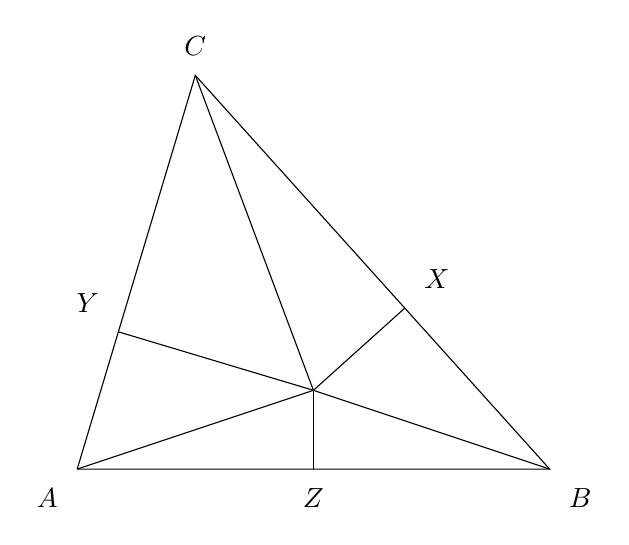
\begin{tikzpicture}

    \coordinate (O) at (0,0);
    \coordinate (A) at (-3,-1);
    \coordinate (B) at (3,-1);
    \coordinate (C) at (-1.5,4);

    \draw (A) -- (B) -- (C) -- (A);
    \foreach \x in {A, B, C}
        \draw (O) -- (\x);
    
    \draw (O) -- ($(A)!(O)!(B)$);
    \draw (O) -- ($(A)!(O)!(C)$);
    \draw (O) -- ($(B)!(O)!(C)$);

    \node[label={south west:$A$}] at (A) {};
    \node[label={south east:$B$}] at (B) {};
    \node[label={above:$C$}] at (C) {};

    \node[label={north east:$X$}] at ($(B)!(O)!(C)$) {};
    \node[label={north west:$Y$}] at ($(A)!(O)!(C)$) {};
    \node[label={south:$Z$}]      at ($(A)!(O)!(B)$) {};

\end{tikzpicture}

            \end{center}
            \label{fig:isosceles_intro}
        \end{figure}


        \begin{enumerate}[(1)]

            \item If $CO$ and $ZO$ do not meet, they are parallel. Therefore
                $CO$ is at right angles to $AB$. Therefore $AC = BC$.

            \item If $CO$ and $ZO$ do meet, let them meet in $O$.  Draw $OX$
                perpendicular to $BC$ and $OY$ perpendicular to $AC$. Join $OA$,
                $OB$.  By Euclid I, 26 (B. and \&., § 88, cor. 7)* the triangles
                $YOC$ and $XOC$ are congruent; also by Euclid I, 47 and I, 8 (B.
                and S., § 156 and § 79)\footnote{These references are to Beman
                and Smith's New Plane and Solid Geometry, Boston, Ginn & Co.,,
                1899.} the triangles $AOY$ and $BOX$ are congruent.  Therefore
                $$AY + YC = BX + XC,$$ i.e., $$AC = BC$$.


                \begin{figure}
                    \label{fig:isosceles_fold}
                    \begin{center}
                        \caption{xx}
                        %% Nice shaded/framed paragraphs using tikz and framed
% Author: Jose Luis Diaz

\begin{tikzpicture}

    \coordinate (O) at (0,0);
    \coordinate (A) at (-3,-1);
    \coordinate (B) at ( 3,-1);
    \coordinate (C) at (-1.5,4);

    \draw (A) -- (B) -- (C) -- (A);
    \foreach \x in {A, B, C}
        \draw (O) -- (\x);
    
    \draw (O) -- ($(A)!(O)!(B)$);

    \node[label={below:$A$}] at (A) {};
    \node[label={below:$B$}] at (B) {};
    \node[label={above:$C$}] at (C) {};

    \node[label={north west:$Z$}] at ($(A)!(O)!(B)$) {};

\end{tikzpicture}


%%%%%%%%%%%%%%%%%%%%%%%%%%%%%%%%%%%%%%%%%%%%%%%%%%%%%%%

% define styles for the normal border and the torn border
\tikzset{
  normal border/.style={orange!30!black!10, decorate,
     decoration={random steps, segment length=2.5cm, amplitude=.7mm}},
  torn border/.style={orange!30!black!5, decorate,
     decoration={random steps, segment length=.5cm, amplitude=1.7mm}}}

% Macro to draw the shape behind the text, when it fits completly in the
% page
\def\parchmentframe#1{
\tikz{
  \node[inner sep=2em] (A) {#1};  % Draw the text of the node
  \begin{pgfonlayer}{background}  % Draw the shape behind
  \fill[normal border]
        (A.south east) -- (A.south west) --
        (A.north west) -- (A.north east) -- cycle;
  \end{pgfonlayer}}}


% Define the environment which puts the frame
% In this case, the environment also accepts an argument with an optional
% title (which defaults to ``Example'', which is typeset in a box overlaid
% on the top border
\newenvironment{parchment}[1][Example]{%
  \def\FrameCommand{\parchmentframe}%
  \def\FirstFrameCommand{\parchmentframetop}%
  \def\LastFrameCommand{\parchmentframebottom}%
  \def\MidFrameCommand{\parchmentframemiddle}%
  \vskip\baselineskip
  \MakeFramed {\FrameRestore}
  \noindent\tikz\node[inner sep=1ex, draw=black!20,fill=white,
          anchor=west, overlay] at (0em, 2em) {\sffamily#1};\par}%
{\endMakeFramed}

%%%%%%%%%%%%%%%%%%%%%%%%%%%%%%%%%%%%%%%%%%%%%%%%%%%%%%%

\newcounter{mathseed}
\setcounter{mathseed}{3}
\pgfmathsetseed{\arabic{mathseed}} % To have predictable results
% Define a background layer, in which the parchment shape is drawn
\pgfdeclarelayer{background}
\pgfsetlayers{background,main}

% This is the base for the fractal decoration. It takes a random point between
% the start and end, and raises it a random amount, thus transforming a segment
% into two, connected at that raised point This decoration can be applied again
% to each one of the resulting segments and so on, in a similar way of a Koch
% snowflake.
\pgfdeclaredecoration{irregular fractal line}{init}
{
  \state{init}[width=\pgfdecoratedinputsegmentremainingdistance]
  {
    \pgfpathlineto{\pgfpoint{random*\pgfdecoratedinputsegmentremainingdistance}{(random*\pgfdecorationsegmentamplitude-0.02)*\pgfdecoratedinputsegmentremainingdistance}}
    \pgfpathlineto{\pgfpoint{\pgfdecoratedinputsegmentremainingdistance}{0pt}}
  }
}


% define some styles
\tikzset{
   
    paper/.style={draw=black!10, blur shadow, 
                  every shadow/.style={opacity=1, black}, 
                  shade=bilinear interpolation, 
                  lower left=black!10, upper left=black!5, 
                  upper right=white, lower right=black!5, 
                  fill=none},

    irregular cloudy border/.style={decoration={irregular fractal line, 
                                    amplitude=0.2}, decorate,},

    irregular spiky border/.style={decoration={irregular fractal line, 
                                   amplitude=-0.2}, decorate,},

    ragged border/.style= {decoration={random steps, segment length=7mm, 
                                       amplitude=2mm}, decorate,}
}

\def\tornpaper#1{

    \ifthenelse{\isodd{\value{mathseed}}}{%
    \tikz{
      \node[inner sep=1em] (A) {#1};  % Draw the text of the node

      \begin{pgfonlayer}{background}  % Draw the shape behind

      \fill[paper] % recursively decorate the bottom border
         \pgfextra{\pgfmathsetseed{\arabic{mathseed}}\addtocounter{mathseed}{1}}
          {decorate[irregular cloudy border]{decorate{decorate{decorate{decorate[ragged border]{
            (A.north west) -- (A.north east)
          }}}}}}
          -- (A.south east)
         \pgfextra{\pgfmathsetseed{\arabic{mathseed}}}%
          {decorate[irregular spiky border]{decorate{decorate{decorate{decorate[ragged border]{
          -- (A.south west)
          }}}}}}
          -- (A.north west);

      \end{pgfonlayer}}
    }

    {
    \tikz{
      \node[inner sep=1em] (A) {#1};  % Draw the text of the node

      \begin{pgfonlayer}{background}  % Draw the shape behind

      \fill[paper] % recursively decorate the bottom border
         \pgfextra{\pgfmathsetseed{\arabic{mathseed}}\addtocounter{mathseed}{1}}%
          {decorate[irregular spiky border]{decorate{decorate{decorate{decorate[ragged border]{
            (A.north east) -- (A.north west)
          }}}}}}
          -- (A.south west)
         \pgfextra{\pgfmathsetseed{\arabic{mathseed}}}%
          {decorate[irregular cloudy border]{decorate{decorate{decorate{decorate[ragged border]{
          -- (A.south east)
          }}}}}}
          -- (A.north east);

      \end{pgfonlayer}}
    }
}

%\tornpaper{ \parbox{.9\textwidth}{\lipsum[11]} }

%\begin{tikzpicture}
%
%    \begin{axis}[colormap/blackwhite, view={30}{60}, axis lines=none]
%
%       \addplot3[surf,shader=interp, samples=60, point meta=x+3*z*z-0.25*y,
%                 domain=0:2*pi,y domain=0:2*pi, z buffer=sort]
%       ({(2+cos(deg(x)))*cos(deg(y))},
%        {(2+cos(deg(x)))*sin(deg(y))},
%        {sin(deg(x))});
%
%   \end{axis}
%
%\end{tikzpicture}

                    \end{center}
                \end{figure}


                Fig.~\ref{fig:isosceles_fold} shows by paper-folding that,
                whatever triangle be taken, $CO$ and $ZO$ cannot meet within the
                triangle.

                $O$ is the mid-point of the arc $AOB$ of the circle which
                circumscribes the triangle $ABC$.

        \end{enumerate}

    \item Paper-folding is not quite foreign to us. Folding paper squares into
        natural objects --- a boat, double boat, ink bottle, cup-plate, etc., is
        well known, as also the cutting of paper in symmetric forms for purposes
        of decoration. In writing Sanskrit and Mahrati, the paper is folded
        vertically or horizontally to keep the lines and columns straight.  In
        copying letters in public offices, an even margin is secured by folding
        the paper vertically.  Rectangular pieces of paper folded double have
        generally been used for writing, and before the introduction of
        machine-cut letter paper and envelopes of various sizes, sheets of
        convenient size were cut by folding and tearing larger sheets, and the
        second half of the paper was folded into an envelope inclosing the first
        half.  This latter process saved paper and had the obvious advantage of
        securing the post marks on the paper written upon.  Paper-folding has
        been resorted to in teaching the XIth Book of Euclid, which deals with
        figures of three dimensions\footnote{See especially Beman and Smith’s
        New Plane and Solid Geometry, p, 287.}.  But it has seldom been used in
        respect of plane figures.


    \item I have attempted not to write a complete treatise or text-book on
        geometry, but to show how regular polygons, circles and other curves can
        be folded or pricked on paper. I have taken the opportunity to introduce
        to the reader some well known problems of ancient and modern geometry,
        and to show how algebra and trigonometry may be advantageously applied
        to geometry, so as to elucidate each of the subjects which are usually
        kept in separate pigeon-holes.


    \item The first nine chapters deal with the folding of the regular polygons
        treated in the first four books of Euclid, and of the nonagon.  The
        paper square of the kindergarten has been taken as the foundation, and
        the other regular polygons have been worked out thereon.  Chapter I
        shows how the fundamental square is to be cut and how it can be folded
        into equal right-angled isosceles triangles and squares.  Chapter II
        deals with the equilateral triangle described on one of the sides of the
        square.  Chapter III is devoted to the Pythagorean theorem (B. and S., §
        156) and the propositions of the second book of Euclid and certain
        puzzles connected therewith.  It is also shown how a right-angled
        triangle with a given altitude can be described on a given base.  This
        is tantamount to finding points on a circle with a given diameter.

    \item Chapter X deals with the arithmetic, geometric, and harmonic
        progressions and the summation of certain arithmetic series.  In
        treating of the progressions, lines whose lengths form a progressive
        series are obtained.  A rectangular piece of paper chequered into
        squares exemplifies an arithmetic series.  For the geometric the
        properties of the right-angled triangle, that the altitude from the
        right angle is a mean proportional between the segments of the
        hypotenuse (B. and.S., § 270), and that either side is a mean
        proportional between its projection on the hypotenuse and the
        hypotenuse, are made use of. In this connexion the Delian problem of
        duplicating a cube has been explained\footnote{See Beman and Smith’s
        translation-of Klein's Famous Problems of Elementary Geometry, Boston,
        1897; also their translation of Fink’s History of Mathematics, Chicago,
        The Open Court Pub. Co., 1900.}  In treating of harmonic progression,
        the fact that the bisectors of an interior and corresponding exterior
        angle of a triangle divide the opposite side in the ratio of the other
        sides of the triangle (B.  and S., § 249) has been used.  This affords
        an interesting method of graphically explaining systems in involution.
        The sums of the natural numbers and of their cubes have been obtained
        graphically, and the sums of certain other series have been deduced
        therefrom.

    \item Chapter XI deals with the general theory of regular polygons, and the
        calculation of the numerical value of $\pi$. The propositions in this
        chapter are very interesting.

    \item Chapter XII explains certain general principles, which have been made
        use of in the preceding chapters, --- congruence, symmetry, and
        similarity of figures, concurrence of straight lines, and collinearity
        of points are touched upon.

    \item Chapters XIII and XIV deal with the conic sections and other
        interesting curves. As regards the circle, its harmonic properties among
        others are treated.  The theories of inversion and co-axial circles are
        also explained.  As regards other curves it is shown how they can be
        marked on paper by paper-folding.  The history of some of the curves is
        given, and it is shown how they were utilised in the solution of the
        classical problems, to find two geometric means between two given lines,
        and to trisect a given rectilineal angle.  Although the investigation of
        the properties of the curves involves a knowledge of advanced
        mathematics, their genesis is easily understood and is interesting.

    \item I have sought not only to aid the teaching of geometry in schools and
        colleges, but also to afford mathematical recreation to young and old,
        in an attractive and cheap form. ``Old boys'' like myself may find the
        book useful to revive their old lessons, and to have a peep into modern
        developments which, although very interesting and instructive, have been
        ignored by university teachers.

\end{enumerate}

\begin{flushright}
{\large T. Sundara Row.\mbox\qquad}\\
\end{flushright}
Madras, India, 1893.

%%%%%%%%%%%%%%%%%%%%%%%%%%%%%%%%%%%%%%%%%%%%%%%%%%%%%%%%%%%%%%%%%%%%%%%%%%%%%%%%


%%%%%%%%%%%%%%%%%%%%%%%%%%%%%%%%%%%%%%%%%%%%%%%%%%%%%%%%%%%%%%%%%%%%%%%%%%%%%%%%

\chapter{THE SQUARE.}

\begin{enumerate}

    \item The upper side of a piece of paper lying flat upon a table is a plane
        surface, and so is the lower side which is in contact with the table.

    \item The two surfaces are separated by the material of the paper. The
        material being very thin, the other sides of the paper do not present
        appreciably broad surfaces, and the edges of the paper are practically
        lines. The two surfaces though distinct are inseparable from each other.

    \item Look at the irregularly shaped piece of paper shown in Fig. 3, and at
        this page which is rectangular. Let us try and shape the former paper
        like the latter.

    \item Place the irregularly shaped piece of paper upon the table, and fold
        it flat upon itself. Let $X'X$ be the crease thus formed. It is
        straight. Now pass a knife along the fold und separate the smaller
        piece.  We thus obtain one straight edge.
    
    \item Fold the paper again as before along $BY$, so that the edge $X'X$ is
        doubled upon itself. Unfolding the paper, we see that the crease $BY$ is
        at right angles to the edge $X'X$. It is evident by superposition that
        the angle $YBX'$ equals the angle $XBY$, and that each of these angles
        equals an angle of the page. Now pass a knife as before along the second
        fold and remove the smaller piece.
    
    \item Repeat the above process and obtain the edges $CD$ and $DA$. It is
        evident by superposition that the angles at $A$, $B$, $C$, $D$, are
        right angles, equal to one another, and that the sides $BC$, $CD$ are
        respectively equal to $DA$, $AB$.  This piece of paper (Fig. 3) is
        similar in shape to the page.
    
    \item It can be made equal in size to the page by taking a larger piece of
        paper and measuring off $AB$ and $BC$ equal to the sides of the latter.
    
    \item A figure like this is called a rectangle.  By superposition it is
        proved that 

        \begin{enumerate}[(1)]
            \item the four angles are right angles and all equal, 
            \item the four sides are not all equal, 
            \item but the two long sides are equal, and so also are the two
                short sides.
        \end{enumerate}

    \item Now take a rectangular piece of paper, $A'B’CD$, and fold it obliquely
        so that one of the short sides, $CD$, falls upon one of the longer
        sides, $DA'$, as in Fig. 4.  Then fold and remove the portion $A'B'BA$
        which overlaps. Unfolding the sheet, we find that $ABCD$ is now square,
        i.e., its four angles are right angles, and all its sides are equal.
    
    
    \item The crease which passes through a pair of the opposite corners $B$,
        $D$, is a diagonal of the square.  One other diagonal is obtained by
        folding the square through the other pair of corners as in Fig. 5.
    
    \item We see that the diagonals are at right angles to each other, and that
        they bisect each other.
    
    \item The point of intersection of the diagonals is called the center of the
        square.
    
    \item Each diagonal divides the square into two congruent right-angled
        isosceles triangles, whose vertices are at opposite corners.
    
    \item The two diagonals together divide the square into four congruent
        right-angled isosceles triangles, whose vertices are at the center of
        the square.
    
    \item \label{item:square} Now fold again, as in Fig. 6, laying one side cf
        the square upon its opposite side. We get a crease which passes through
        the center of the square. It is at right angles to the other sides and 

    \begin{enumerate}[(1)]
        \item bisects them; 
        \item it is also parallel to the first two sides; 
        \item it is itself bisected at the center; 
        \item it divides the square into two congruent rectangles, which are,
            therefore, each half of it; 
        \item each of these rectangles is equal to one of the triangles into 
            which either diagonal divides the square.
    \end{enumerate}

    \item Let us fold the square again, laying the remaining two sides one upon
        the other. The crease now obtained and the one referred to in
        \ref{item:square} divide the square into four congruent squares.
    
    \item Folding again through the corners of the smaller squares which are at
        the centers of the sides of the larger square, we obtain a square which
        is inscribed in the latter. (Fig. 7.)
    
    \item This square is half the larger square, and has the same center.
    
    \item By joining the mid-points of the sides of the inner square, we obtain
        a square which is one-fourth of the original square (Fig. 8). By
        repeating the process, we can obtain any number of squares which are to
        one another as $$\frac{1}{2},  \frac{1}{4}, \frac{1}{8},
        \frac{1}{16}, \text{etc., or } \frac{1}{2}, \frac{1}{2^2},
        \frac{1}{2^3}, \frac{1}{2^4}, \cdots$$

        Each square is half of the next larger square, i.e., the four triangles
        cut from each square are together equal to half of it. The sums of all
        these triangles increased to any number cannot exceed the original
        square, and they must eventually absorb the whole of it.

        Therefore $$\frac{1}{2} + \frac{1}{2^2} + \frac{1}{2^3} + \text{etc.\ to
        infinite} = 1$$.


    \item The center of the square is the center of its circumscribed and
        inscribed circles. The latter circle touches the sides at their
        mid-points, as these are nearer to the center than any other points on
        the sides.

    \item Any crease through the center of the square divides it into two
        trapezoids which are congruent. A second crease through the center at
        right angles to the first divides the square into four congruent
        quadrilaterals, of which two opposite angles are right angles.  The
        quadrilaterals are concyclic, i.e., the vertices of each lie in a
        circumference.

\end{enumerate}

% i am here
%%%%%%%%%%%%%%%%%%%%%%%%%%%%%%%%%%%%%%%%%%%%%%%%%%%%%%%%%%%%%%%%%%%%%%%%%%%%%%%%

%%%%%%%%%%%%%%%%%%%%%%%%%%%%%%%%%%%%%%%%%%%%%%%%%%%%%%%%%%%%%%%%%%%%%%%%%%%%%%%%

\chapter{THE EQUILATERAL TRIANGLE.}


\begin{enumerate}

    \item Now take this square piece of paper (Fig. 9), and fold it double,
        laying two opposite edges one upon the other. We obtain a crease which
        passes through the mid-points of the remaining sides and is at right
        angles to those sides.  Take any point on this line, fold through it and
        the two corners of the square which are on each side of it. We thus get
        isosceles triangles standing on a side of the square.
    
%Fig. 9.  Fig. 10.  Fig. 11.

    \item The middle line divides the isosceles triangle into two congruent
        right-angled triangles.
    
    \item The vertical angle is bisected.
    
    \item If we so take the point on the middle line, that its distances from
        two corners of the square are equal to a side of it, we shall obtain an
        equilateral triangle (Fig. 10).  This point is easily determined by
        turning the base $A$ through one end of it, over $AA'$, until the other
        end, $B$, rests upon the middle line, as at $C$.
    
    \item Fold the equilateral triangle by laying each of the sides upon the
        base.  We thus obtain the three altitudes of the triangle, viz.: $AA'$,
        $BB'$, $CC'$, (Fig.  11).
    
    \item Each of the altitudes divides the triangle into two congruent
        right-angled triangles.

    \item They bisect the sides at right angles.

    \item They pass through a common point.

    \item Let the altitudes $AA'$ and $CC'$ meet in $O$.  Draw $BO$ and produce
        it to meet $AC$ in $B'$.  $BB'$ will now be proved to be the third
        altitude.  From the triangles $C'OA$ and $COA'$, $OC'=OA'$.  From
        triangles $OC'B$ and $A'OB$, $\angle OBC'= \angle A'BO$.  Again from
        triangles $ABB'$ and $CB'B$, $\angle AB'B = \angle BB'C$, i.e., each of
        them is a right angle.  That is, $BOB'$ is an altitude of the
        equilateral triangle $ABC$.  It also bisects $AC$ in $B'$.

    \item It can be proved as above that $OA$, $OB$, and $OC$ are equal, and
        that $OA'$, $OB'$, and $OC'$ are also equal.

    \item Circles can therefore be described with $O$ as a center and passing
        respectively through $A$, $B$, and $C$ and through $A'$, $B'$, and $C$.
        The latter circle touches the sides of the triangle.
    
    \item The equilateral triangle $ABC$ is divided into six congruent
        right-angled triangles which have one set of their equal angles at $O$,
        and into three congruent, symmetric, concyclic quadrilaterals.

    \item The triangle $AOC$ is double the triangle $A'OC$; therefore, $AO = 2
        OA'$.  Similarly, $BO=2OB'$ and $CO=2OC'$. Hence the radius of the
        circumscribed circle of triangle ABC is twice the radius of the
        inscribed circle.
    
    \item The right angle $A$, of the square, is trisected by the straight lines
        $AO$, $AC$.  Angle $BAC = \frac{2}{3}$ of a right angle. The angles
        $C'AO$ and $OABD'$ are each $\frac{1}{3}$ of a right angle.  Similarly
        with the angles at $B$ and $C$.

    \item The six angles at $O$ are each $\frac{2}{3}$ of a right angle.
    
    \item Fold through $A'B'$, $BC'$, and $C'A'$ (Fig. 12).  Then $A'B'C'$ is an
        equilateral triangle.  It is a fourth of the triangle $ABC$.
    
    \item $A'B'$, $B'C'$, $C'A'$ are each parallel to $AB$, $BC$, $CA$, and
        halves of them.
    
    \item $AC'A'B'$ is a rhombus. So are $C'BA'B'$ and $CB'C'A'$.
    
    \item $A'B'$, $B'C'$, $C'A'$ bisect the corresponding altitudes.
    
    \item $CC'^{2} + AC'^{2} =  CC'^{2} + \frac{1}{4} AC^{2} = AC^{2}$\\
        $\therefore CC'^{2} = \frac{3}{4} AC^{2}$\\
        $\therefore CC' = \frac{1}{2} \sqrt{3} \cdot AC = \frac{1}{2} \sqrt{3}
        \cdot AB $\\
        $ = 0.866\ldots \times AB$.
    
    %Fig. 12.
    
    \item The $\triangle ABC =$ rectangle of $AC'$ and $CC'$, i.e.\ $\frac{1}{2}
        AB \times \frac{1}{2} \sqrt{3} \cdot AB = \frac{1}{4} \sqrt{3} \cdot
        AB^{2} = 0.433\ldots \times AB^{2}$.
    
    \item The angles of the triangle $AC'C$ are in the ratio of $1:2:3$, and its
        sides are in the ratio of $\sqrt{1}:\sqrt{3}:\sqrt{4}$.

\end{enumerate}

%%%%%%%%%%%%%%%%%%%%%%%%%%%%%%%%%%%%%%%%%%%%%%%%%%%%%%%%%%%%%%%%%%%%%%%%%%%%%%%%

%%%%%%%%%%%%%%%%%%%%%%%%%%%%%%%%%%%%%%%%%%%%%%%%%%%%%%%%%%%%%%%%%%%%%%%%%%%%%%%%

\chapter{SQUARES AND RECTANGLES.}


\begin{enumerate}

    \item Fold the given square as in Fig. 13. This affords the well-known proof
        of the Pythagorean theorem.  $FGH$ being a right-angled triangle, the
        square on $FH$ equals the sum of the squares on $FG$ and $GH$.

        $$\square FA + \square DB = \square FC$$.

        It is easily proved that $FC$ is a square, and that the triangles $FGH$,
        $HBC$, $KDC$, and $FEK$ are congruent.

        If the triangles $FGH$ and $HBC$ are cut off from the squares $FA$ and
        $DB$, and placed upon the other two triangles, the square $FHCK$ is made
        up.

%If 4B=2, GA=d, and FH=c, then.2 += 2’.

    \item Fold the given square as in Fig. 14. Here the rectangles 47, $BG$,
        $CH$, and $DE$ are congruent, as also the triangles of which they are
        composed.  $E7XGH$ is a square as also $KZMN$.

%et 4k ——2,14h eb =>, and Vk =<,
%
%then a?+ 2?=—¢?, i.e. 0OKLMN.
%
%oABCD=(a- 4).  Now square ABCD overlaps the square KLMN by the four triangles
%AK, BLK, CML, and DNM.  But these four triangles are together equal to
%two of the rectangles, i.  e., to 2aé.  Therefore (a+ 0)? =a? + 6? + 2ad.
%
%
%\item EF=—a—dé, ando EFGH= (a—)’.  The square £¥G/H is less
%than the square AL MN by the four triangles PVK, GAL, HLM, and EMN.
%But these four triangles make up two of the rectangles, i. e., 2ad.
%.t. (a—b)? =a? + 6? — 2adb.
%
%Fig. 15 Fig. 16.  Fig. 17.
%
%
%\item The square ABCD overlaps the square E¥GH by the four rectangles 4/7,
%BG, CH, and DE.  .. (a+ 4)? — (a—b)? =4ab.
%
%\item In Fig. 15, the square 4BCD=(a- 6)’, and the square
%-F¥GH=(a—d)*. Also square AKGN = square EZLCM=a*. Square KBLF = square
%NHMD = 0’.
%
%Squares ABCD and EFGH are together equal to the latter four squares put
%together, or to twice the square d4XGW and twice the square KBLF, that is,
%
%(a+ 4)? + (a— 4)? = 2a? + 207.
%
%
%\item In Fig. 16 the rectangle PZ is equal to (a+ 4) (@—2).
%
%Because the rectangle EX — FM, therefore rectangle PZ = square PAX
%—square A#, i. e., (a+) (a— 6) =a? — 3b.

    \item If squares be described about the diagonal of a given square, the
        right angle at one corner being common to them, the lines which join
        this corner with the mid-points of the opposite sides of the given
        square bisect the corresponding sides of all the inner squares. (Fig.
        17.) For the angles which these lines make with the diagonal are equal,
        and their magnitude is constant for all squares, as may be seen by
        superposition. Therefore the mid-points of the sides of the inner
        squares must lie on these lines.

    \item $ABCD$ being the given square piece of paper (Fig. 18), it is required
        to obtain by folding, the point $X$ in $AB$, such that the rectangle
        $AB-XVP$ is equal to the square on $AX$.

        Double $AC$ upon itself and take its mid-point $Z$.

        Fold through $Z$ and $4$.

%Lay £B upon £A and fold so as to get £F, and G such that EG=£B.
%
%Take AX= AG.
%
%Then rectangle 4B: XB=AX’”.
%
%Complete the rectangle BCHX and the square AXKL.
%
%Let XH cut HA in MW. Take FY=/FB.
%
%Then FB =/G=FY=XM and XM=4AX,
%
%Fig. 18.
%
%Now, because #Y is bisected in # and produced to A, AB:AY+ FY°=AF”,
%by § 49, =AG?+ FG", by § 44.  siete AY a A, oe ks But AX* 224° NA on B 4,
%
%24 AX DY and Ay AX, sn ABN BAN es AB is said to be divided in X in median
%section. * Also AB-AY=BY%*, i. e., 4B is also divided in Y in median section.
%
    
    \item A circle can be described with $F$ as a center, its circumference
        passing through $A$, $G$, and Y.  It will touch $ZA$ at $G$, because 
        $/G$ is the shortest distance from F to the line $EGA$.

%\item Since BH=BN, subtracting BX we have rectangle XX/VY = square CHP,
%i. e., AX: YX=AY?,
%
%i. e., AX is divided in Y in median section.  Similarly AY is divided in
%X in median section.  54. °.: 4B: XB=AX?
%
%.. 84B:-XB=AX?+ BX:-BC+ CD-CP — ABI + BX?,
%
%\item Rectangles BH and YD being each=AB- XB, rectangle HY + square CK =
%AX? = AB: XB.
%
%\item Hence rectangle 7Y= rectangle BK, i. e., AX: XB=AB:XY.
%
%\item Hence rectangle HV=AX:-XB— BX?.
%
%*The term “ golden section” is also used. See Beman and Smith's Vew
%Plane and Solid Geometry, p. 196.
%
%\item Let A4B=a, XB =x.  Then (a— x)? =ax, by § 51.  a? + x? —3ax,
%by § 54;
%
%and =F (3—V5).  ao : esta nae: =z (7—3V'5).
%
%
%a x= 5 (VbB—1) =a X 0.6180...
%
%
%2 = +. (@—x) =F (83— V5) =a? x 0.3819...  The rect. BPAX = (a—x)x
%=a? (V5—2)=a’x0.2360....  EA'=5sEB? — 3 AB BA = 4B =1.1180. eo.
%
%
%\item In the language of proportion AD AX aA Kae XB The straight line 4B is
%said to be divided ‘in extreme and mean ratio.”

    \item Let $AZ$ be divided in $X$ in median section.  Complete the rectangle
        $CBXH$ (Fig.  19).  Bisect the rectangle by the line $A/VO$. Find the
        point $WV$ by laying $XA$ over $X$ so that $A$ falls on $AZO$, and fold
        through $XV$, $VB$, and $VA$.  Then $BAW$ is an isosceles triangle
        having its angles $AB$ and $BNA$ double the angle $VAB$.

%AX=AN=NLB LABN=ZNXB LINNAX== SANA LNXB=2/NAX
%
%Fig. 19.
%
%
%L ABN=2/ NAB.  AN*=MN?4+ AM?
%
%— BN*—BM?+ AM?
%
%—AX2+4 AB-AX
%
%—AB-XB1+AB:AX
%
%— AB?
%
%<i AVA, and LNAB =} of a right angle.
%
%
%\item The right angle at 4 can be divided into five equal parts as in Fig. 20.
%Here WV’ is found as in § 60. Then fold AW'Q; bisect / QAB by folding,
%fold over the diagonal AC and thus get the point ks
%
%A B
%
%
%Fig. 20.
%
%\item To describe a right-angled triangle, given the hypotenuse 4BZ, and
%the altitude.
%
%Fold £F (Fig. 21) paraHel to AB at the distance of the given altitude.
%
%Take G the middle point of 42. Find # by folding GB through G so that B
%may fall on 2/.
%
%Fold through H and 4, G, and B.  AB is the triangle required.
%
%Fig. 2r.
%

    \item $ABCD$ (Fig: 22) is a rectangle.  It is required to find a square
        equal to it in area.

%Mark off B= BC.  Find O, the middle point of 4J/, by folding.

%Fold OM, keeping O fixed and letting J/ fall on line BC, thus finding /,
%the vertex of the right-angled triangle 41/P.
%
        Describe on $PB$ the square $BPQOR$.

%The square is equal to the given rectangle. |
%
%For -.3P=QP, and the angles are equal, triangle BMP is evidently congruent
%to triangle QSP.
%
%eto == DM == AD.
%
%.*. triangles DA 7 and QSP are congruent.
%
%... PC=SR and triangles RSA and CPT are congruent.
%
%.*. [ABCD can be cut into three parts which can be fitted together to form
%the square RAPQ.
%
%Fig. 23 Fig. 24.  Fig. 25.

    \item Take four equal squares and cut each of them into two pieces through
        the middle point of one of the sides and an opposite corner. Take also
        another equal square. The eight pieces can be arranged round the square
        so as to form a complete square, as in Fig.  23, the arrangement being a
        very interesting puzzle.  The fifth square may evidently be cut like the
        others, thus complicating the puzzle.  

    \item Similar puzzles can be made by cutting the squares through one corner
        and the trisection points of the opposite side, as in Fig.  24.  areas

    \item If the nearer point is taken 10 squares are required, as in Fig. 24;
        if the remoter point is taken 13 squares are required, as in Fig. 25.  

    \item The puzzles mentioned in §§ 65, 66, are based upon the formulas

%12+ 2?—=5 124+ 3710 22.4 3? — 13.

        The process may be continued, but the number of squares will become
        inconveniently large.

    \item Consider again Fig. 13 in § 44. If the four triangles at the corners
        of the given square are removed, one square is left. If the two
        rectangles $XK$ and $XG$ are removed, two squares in juxtaposition are
        left.

    \item The given square may be cut into pieces which can be arranged into two
        squares.  There are various ways of doing this. Fig. 23, in § 65,
        suggests the following elegant method: The required pieces are 

        \begin{enumerate}[(1)]
            \item the square in the center, and 
            \item the four congruent symmetric quadrilaterals at the corners,
                together with the four triangles. 
        \end{enumerate}
    
        In this figure the lines from the mid-points of the sides pass through
        the corners of the given square, and the central square is one-fifth of
        it. The magnitude of the inner square can be varied by taking other
        points on the sides instead of the corners.

    \item The given square can be divided as follows (Fig. 26) into three equal
        squares: Take $BG = \text{half the diagonal of the square}$.

%Fig. 26.

    Fold through C and G.

    Fold BM perpendicular to CG.

    Take MP, CN, and VZ each = BM.
    
    Fold PH, NX, ZF at right angles to CG, as in Fig. 26.
    
    Take VK = BM, and fold K£ at right angles to NE.
    
    Then the pieces 1, 4, and 6, 3 and 5, and 2 and 7 form three equal squares.
    
    Now CG?=3BG’, and from the triangles GBC and CVB BM BG.  Pieris
    
    Letting BC—=a, we have
    
\end{enumerate}

%%%%%%%%%%%%%%%%%%%%%%%%%%%%%%%%%%%%%%%%%%%%%%%%%%%%%%%%%%%%%%%%%%%%%%%%%%%%%%%%

%%%%%%%%%%%%%%%%%%%%%%%%%%%%%%%%%%%%%%%%%%%%%%%%%%%%%%%%%%%%%%%%%%%%%%%%%%%%%%%%

\chapter{THE PENTAGON.}

\begin{enumerate}

    \item To cut off a regular pentagon from the square ABCD. 7

        Divide $BA$ in $X$ in median section and take $YW$ the mid-point of
        $4X$.

%Fig. 27.
%
%Then 4B: AX=XB?, and AM= MX.
%
%Take BVN=AM or MX.
%
%Then MV= XB.
%
%Lay off VP and WR equal to AZN, so that P and R may lie on BC and AD
%respectively.
%
%Lay off RQ and PO=WMR and WP.
%
%MNPOQR is the pentagon required.
%
%In Fig. 19, p. 22, 4, which is equal to 4B, has the point JV on the
%perpendicular 7O. If A be moved on AB over the distance 7A, then it is
%evident that JV will be moved on to BC, and X to
%
%Therefore, in Fig. 27, VR=AB. Similarly “P= AB. RP is also equal to AZ
%and parallel to it.
%
%LRMA =} of a tt. /.  we dV A ee Ola ttf
%
%Similarly LENM =F ofa tt. 2. .
%
%From triangles VR and QORP, 7 NMR= 7 ROP == of a rt. 7.
%
%The three angles at 17, 4, and Q of the pentagon being each equal to § of
%a right angle, the remaining two angles are together equal to 12 of a right
%angle, and they are equal. Therefore each of them is £ of a right angle.
%
%Therefore all the angles of the pentagon are equal.
%
%The pentagon is also equilateral by construction.
%
%was ae base AZZ of the pentagon is equal to XB, og ees Bay
%5—1)=ABX0.6180.... § 58.  The sie test breadth of the pentagon is 4B.
%
%
%\item If p be the altitude, 2 AB = pr Es vWe— 1)| 51/5.  eee Sa —V 5.
%-paap.(1—8 | — pe PTV S 8 V 2V5 Sn af eerie dee se a == ABO 2510. cane A Cos 18,
%
%AY
%
%
%Fig. 28.
%
%\item If & be the radius of the circumscribed circle,
%
%‘AB eee ~ 2cos18° 104275 5— V5.  aera
%
%
%— AB 0.5257...
%
%\item If r be the radius of the inscribed circle, then from Fig. 28 it is
%evident that
%
%
%Pops Re ABs cote — AB: pice =AB+V/b4+V5. (J 3 +425") =4n-Voqve [oe
%
%
%Vv 40 Legs ses
%
%
%=AB 0.4203 556 76. The area of the pentagon is 57 x } the base of the
%pentagon, i. e.,
%
%
%[545 | au
%
%
%Bea -(V5—1)
%
%
%5 22 =A —jo = 4B X 0.6571...
%
%
%\item In Fig. 27 let PR be divided by WQ and VQ in £ and /.
%
%
%%Then MN= 22 (5-1). $72
%
%
%Pee ee ee eee pe ot 2 cos 36° SSE =o eet a
%
%EF=AB—2RE=AB—AB(3—V 5) =AB(V5—2)... (2)
%
%
%RF=MN.  RF: RE == RE» EF (by § 51)... 0.52202 eens en cease Y6—173 V6
%=3—Y 5: 2(V 6 —2).. ie venene (4) By § 76 the area of the pentagon 5
%[5—V5 VeHiv 8 obeys Sas 7. pi tose C8 pe A =a -( 2 4 10 = MN: 1/25 +
%10V5, since AB= un yes
%
%
%.'. the area of the inner pentagon = EF?4 : oes 10V5 = AB (Y5—2) +
%5 1 1/2 +105.
%
%
%The larger pentagon divided . the smaller = MN? : EF?  =2:(7T—3Vv 5)
%=1 : 0.145898...
%
%\item If in Fig. 27, angles QEX and ZFOQ are made equal to 2RQ or FOP, K, Z
%being points on the sides QR and QP respectively, then EFL QK will be a regular
%pentagon congruent to the inner pentagon. Pentagons can be similarly described
%on the remaining sides of the inner pentagon. The resulting figure consisting of
%six pentagons is very interesting.
%
\end{enumerate}

%%%%%%%%%%%%%%%%%%%%%%%%%%%%%%%%%%%%%%%%%%%%%%%%%%%%%%%%%%%%%%%%%%%%%%%%%%%%%%%%

%%%%%%%%%%%%%%%%%%%%%%%%%%%%%%%%%%%%%%%%%%%%%%%%%%%%%%%%%%%%%%%%%%%%%%%%%%%%%%%%

\chapter{THE HEXAGON.}


\begin{enumerate}

\item To cut off a regular hexagon from a given square.  Fold through the
    mid-points of the opposite sides, and obtain the lines 408 and COD.

%Fig. 29.

    On both sides of $AO$ and $OB$, describe equilateral triangles (§ 25),
    $AOL$, $AHO$; $BFO$ and $BOG$.

    Draw $EF$ and $HG$.

    $AHGSFE$ is a regular hexagon.

    It is unnecessary to give the proof.

    The greatest breadth of the hexagon is 4.


\item The altitude of the hexagon is
%
%
%V 3 BEER EE
%
%
%Fig. 30.
%

\item If R be the radius of the circumscribed circle,


%1 R=; AB.
%

\item If be the radius of the inscribed circle,


%3 ra! AB=0.433....X AB,


\item The area of the hexagon is 6 times the area of the triangle HGO,


%AB V3 ae 1s -AB?=0.6495....< AB?  Also the hexagon = 3: AB:CD.


%= 1} times the equilateral triangle on 4B.

%Fig. 31.



\item Fig. 30 is an example of ornamental folding into equilateral triangles and
    hexagons.

\item A hexagon is formed from an equilateral triangle by folding the three
    corners to the center.  The side of the hexagon is 4 of the side of the
    equilateral triangle.

    The area of the hexagon = 3 of the equilateral triangle.

\item The hexagon can be divided into equal regular hexagons and equilateral
    triangles as in Fig. 31 by folding through the points of trisection of the
    sides.

\end{enumerate}

%%%%%%%%%%%%%%%%%%%%%%%%%%%%%%%%%%%%%%%%%%%%%%%%%%%%%%%%%%%%%%%%%%%%%%%%%%%%%%%%

%%%%%%%%%%%%%%%%%%%%%%%%%%%%%%%%%%%%%%%%%%%%%%%%%%%%%%%%%%%%%%%%%%%%%%%%%%%%%%%%

\chapter{THE OCTAGON.}


\begin{enumerate}

    \item To cut off a regular octagon from a given square.  Obtain the
        inscribed square by joining the mid-points $A,$, $B,$, $C,$, $D$ of the
        sides of the given square.

%Fig. 32.

        Bisect the angles which the sides of the inscribed square make with the
        sides of the other. Let the bisecting lines meet in Z. /, G, and ZH.

        $AEBFCGDA$ is a regular octagon.
    
        The triangles $AEB$, $BFC$, $CGD$, and $DHA$ are congruent isosceles
        triangles.  The octagon is therefore equilateral.
    
        The angles at the vertices, Z, 7, G, H of the same four triangles are
        each one right angle and a half, since the angles at the base are each
        one-fourth of a right angle.
    
        Therefore the angles of the octagon at A, B, C, and D are each one right
        angle and a half.
    
        Thus the octagon is equiangular.
    
        The greatest breadth of the octagon is the side of the given square, a.
    
    \item If \& be the radius of the circumscribed circle, and a be the side of
        tke original square, a
    
    \item The angle subtended at the center by each of the sides is half a right
        angle.
    
    
    \item Draw the radius $OB$ and let it cut $AB$ in $K$ (Fig. 33).
    
%Then AK = OK= C4 wh V 2 2V 2 rT as a oe i ae =< KE=04A—0OK=5 Rare V2).
%
%
%Now from triangle 474, AP=—AK%+ KF @
%
%
%Ee eee ooo 2/2 =3 1 3) Soe
%
%a — = g (4—2V2) a =~
%
%S
%
%
%AB= 5 VY 2—V2.
%
%
%g1. The altitude of the octagon is CZ (Fig. 33).  But CH? —=AC*—_ AF a > a =
        %=@_— 7+ Q—V2)=7-2+V2).  c
%
%
%DS MDE
%
%
%ANG
%
%
%Fig. 33.
%
%
%eae lt Be Wa
%
%
%2
%
%
    \item The area of the octagon is eight times the triangle $AOE$ and
%
%
%2 Bede feed a 2 32 v2

    \item A regular octagon may also be obtained by dividing the angles of the
        given square into four equal parts.


%<I YS yo
%
%
%Ww K Fig. 34.
%
%
%
%It is easily seen that EZ= WZ—=a, the side of the square. .  XZ=aV2;
    %XE=a(V2—1); XE=WH=-WEK: KX =a—a(V2—1) —a(2—V2).  Now KZ?=a?4+ a2(V2—1)? =a?
    %(4—2V2) . KZ=aV 4—2V2.  Also GE =XZ—2XE =aV 2—2a(V2— 1)
%
%
%=a(2—V 2).
%
%+. HO=5 (2-V2).  Again 0Z=5V2, and HZ?— HO*?+ OZ?  =" (6—4V242)
%
%
%=a? (2—/Y2).  2. AZ=et/ 2—72.
%
%
%HK = KZ— HZ at|y t-29 2 —a|/ ov 2 en(/ 2-72 )c Vv 2—1)
%
%
%=aVy10—TV2.  1 : “1 /i0_ Ty 2.  and HA=SV2—14V2.
%
%
\item The area of the octagon is eight times the area of the triangle $HOA$,
%
%
%Bra V2
%
%
%%= HO? 2/2 =|$(@—-v2) ):2v2 —7-2V2-(6—4V2)
%
%
%=a? (3V2—4) =a?-V2-(V2—1)?.
%
%
%, aS “oka re?) .  cv 5 ate ‘ 7 a? a Lar 7 7 .  or . * 44 GEOMETRIC EXERCISES
%
%
%\item This octagon: the octagonin§ 92 — = (2—V2)?:1 or 2:(V24 1); and their
    %bases are to one another as
%
%
%a vo se
%
\end{enumerate}


%%%%%%%%%%%%%%%%%%%%%%%%%%%%%%%%%%%%%%%%%%%%%%%%%%%%%%%%%%%%%%%%%%%%%%%%%%%%%%%%

%%%%%%%%%%%%%%%%%%%%%%%%%%%%%%%%%%%%%%%%%%%%%%%%%%%%%%%%%%%%%%%%%%%%%%%%%%%%%%%%

\chapter{THE NONAGON.}

\begin{enumerate}

\item Any angle can be trisected fairly accurately by paper folding, and in this
    way we may construct approximately the regular nonagon.

%Fig. 35.
    
    Obtain the three equal angles at the center of an equilateral triangle. (§
    25.)

    For convenience of folding, cut out the three angles, $AOF$, $FOC$, and
    $COA$.  Trisect each of the angles as in Fig. 35, and make each of the arms 
    $OA$.


\item Each of the angles of a nonagon is 1,4 of a right angle — 140°.

    The angle subtended by each side at the center is 4 of a right angle or 40°.


    Half this angle is 4 of the angle of the nonagon.


\item $OA = ha$, where $a$ is the side of the square; it is also the radius of
    the circumscribed circle, 2.  The radius of the inscribed circle $= A . cos
    20°$


%= 4a cos 20° = © x0.9396926 =a X 0.4698463.  The area of the nonagon is 9 times
%the area of the triangle AOL = 9-R-4R sin 40° $ R?-sin 40°
%
%
%9a2 <0. 6427876
%
%|
%
%
%I
%
%
%—= a? 0.723136,
%
\end{enumerate}

%%%%%%%%%%%%%%%%%%%%%%%%%%%%%%%%%%%%%%%%%%%%%%%%%%%%%%%%%%%%%%%%%%%%%%%%%%%%%%%%

%%%%%%%%%%%%%%%%%%%%%%%%%%%%%%%%%%%%%%%%%%%%%%%%%%%%%%%%%%%%%%%%%%%%%%%%%%%%%%%%

\chapter{THE DECAGON AND THE DODECAGON.}



\begin{enumerate}

\item Figs. 36, 37 show how a regular decagon, and a regular dodecagon, may be
    obtained from a pentagon and hexagon respectively.

%
%Fig. 36.
%
%
    The main part of the process is to obtain the angles at the center.

    In Fig. 36, the radius of the inscribed circle of the pentagon is taken for
    the radius of the circumscribed circle of the decagon, in order to keep it
    within the square.

\item A regular decagon may also be obtained as follows:

    Obtain $X$, $Y$, (Fig. 38), as in § 51, dividing $A$ in median section.

    Take $X$ the mid-point of $AB$.

    Fold $XC$, $WO$, $YD$ at right angles to $AB$.

    %Take -O in WO such that VYO=AY, or YO=XB.

%Fig. 37.


    Let $YO$, and $XO$ produced meet $XC$, and $YD$ in $C$ and $D$ respectively.

    Divide the angles $XOC$ and $DOY$ into four equal parts by $HOZL$, $KOF$, 
    and $LOG$.

    Take $OH$, $OK$, $OL$, $OF$, $OF$, and $OG$ equal to $OY$ or $OX$.

    Join $X$, $H$, $K$, $LZ$, $C$, $D$, $£$, $G$, and $Y$, in order.

    %As in § 60, LVOXS¢ of att. 736"

%Fig. 38.

    By bisecting the sides and joining the points thus determined with the
    center, the perigon is divided into sixteen equal parts. A $16$-gon is
    therefore easily constructed, and so for a $32$-gon, and in general a
    regular $2^n$-gon.
    
\end{enumerate}

%%%%%%%%%%%%%%%%%%%%%%%%%%%%%%%%%%%%%%%%%%%%%%%%%%%%%%%%%%%%%%%%%%%%%%%%%%%%%%%%

%%%%%%%%%%%%%%%%%%%%%%%%%%%%%%%%%%%%%%%%%%%%%%%%%%%%%%%%%%%%%%%%%%%%%%%%%%%%%%%%

\chapter{THE PENTEDECAGON.}


\begin{enumerate}

\item Fig. 39 shows how the pentedecagon is obtained from the pentagon.  Let
    $ABCDE$ be the pentagon and $QO$ its center.

%
%
%JR
%
%Dal VAY TIES
%
%
%Fig. 39.

    Draw $OA$, $OB$, $OC$, $OD$, and $OZ$. Produce $DO$ to meet $AZ$ in $K$.

%Take OF =} of OD.

    Fold $GFA$ at right angles to $OF$. Make $OG= OH = OD$.

    Then $GDA$ is an equilateral triangle, and the angles $DOG$ and $HOD$ are
    each $120°$

    But angle $DOA$ is $144°$; therefore angle $GOA$ is $24°$,

    That is, the angle $HOA$, which is $72°$, is trisected by $OG$.

    Bisect the angle $HOG$ by $OZ$, meeting $ZA$ in $Z$, and let $OG$ cut $EA$
    in $WM$; then

%OL=OM.
%
    In $OA$ and $OF$ take $OP$ and $OQ$ equal to $OZ$ or $OM$.

    Then $PM$, $MZ$, and $ZQ$ are three sides of the pentedecagon.

    Treating similarly the angles $AOB$, $BOC$, $COD$, and $DOZ$, we obtain the
    remaining sides of the pentedecagon.

\end{enumerate}


%%%%%%%%%%%%%%%%%%%%%%%%%%%%%%%%%%%%%%%%%%%%%%%%%%%%%%%%%%%%%%%%%%%%%%%%%%%%%%%%

%%%%%%%%%%%%%%%%%%%%%%%%%%%%%%%%%%%%%%%%%%%%%%%%%%%%%%%%%%%%%%%%%%%%%%%%%%%%%%%%

\chapter{SERIES.}


%%%%%%%%%%%%%%%%%%%%%%%%%%%%%%%%%%%%%%%%

ARITHMETIC SERIES.


\begin{enumerate}

\item Fig. 40 illustrates an arithmetic series. The horizontal lines to the left
    of the diagonal, including the upper and lower edges, form an arithmetic
    series.


%SY a ae a4 ee
%
%dS ee ee
%
%
%Fig. 40.
%
%
%The initial line being a, and d the common difference, the series is a, a+ d,
        %a+ 2d, a+ 3d, etc.
%

\item The portions of the horizontal lines to the right of the diagonal also
    form an arithmetic series, but they are in reverse order and decrease with a
    common difference.


\item In general, if / be the last term, and s the sum of the series, the above
    diagram graphically proves the formula n

%s=—5 (a+7).  105. If @ and ¢ are two alternate terms, the middle term is ate a
%

\item To insert z means between a and /, the vertical line has to be folded into
    + 1 equal parts. The common difference will be

%/—a a+1° 107. Considering the reverse series and interchanging a and /, the
        %series becomes a, @—d, @Q—2a..../.  The terms will be positive so long
        %as a>(a—1)d, and thereafter they will be zero or negative.

%%%%%%%%%%%%%%%%%%%%%%%%%%%%%%%%%%%%%%%%

GEOMETRIC SERIES.


\item In a right-angled triangle, the perpendicular from the vertex on the
    hypotenuse is a geometric mean between the segments of the hypotenuse.
    Hence, if two alternate or consecutive terms of a geometric series are
    given in length, the series can be determined as in Fig. 41. Here OP,
    OP2, OP, OPs, and OP; form a geometric series, the common rate being OP;
    : OP


%Ps
%
%
%Fig. 41.


    If OP; be the unit of length, the series consists of the natural powers of
    the common rate.


%\item Representing the series by a, ar, ar?,....  Pi Py =aV 1 +r.  P, P3=arV1+
        %7.  P3; Ps=ar*) fT + 73,
%
%
These lines also form a geometric series with the common rate ”.


\item The terms can also be reversed, in which case the common rate will be a
    proper fraction. If OP be the unit, OP; is the common rate. The sum of the
    series to infinity is OP;


%OP; — OP,

\item In the manner described in § 108, one geometric mean can be found between
    two given lines, and by continuing the process, $3$, $7$, $15$, etc., means
    can be found. In general, 2*—-1 means can be found, $m$ being any positive
    integer.


\item It is not possible to find two geometric means between two given lines,
    merely by folding through known points. It can, however, be accomplished in
    the following manner: In Fig. 41, OP; and OF, being given, it is required to
    find P, and P3. Take two rectangular pieces of paper and so arrange them,
    that their outer edges pass through 7; and /4, and two corners lie on the
    straight lines OP; and OP; in such a way that the other edges ending in
    those corners coincide.

    The positions of the corners determine OP: and OP3.


\item This process gives the cube root of a given number, for if OP, is the
    unit, the series is 1, 7, 7?, 7°.


\item There is a very interesting legend in connection with this problem. ''The
    Athenians when suffering from the great plague of eruptive typhoid fever in
    430 B.C., consulted the oracle at Delos as to how they could stop it.
    Apollo replied that they must double the size of his altar which was in the
    form of a cube.  Nothing seemed more easy, and a new altar was constructed
    having each of its edges double that of the old one.  The god, not
    unnaturally indignant, made the pestilence worse than before.  A fresh
    deputation was accordingly sent to Delos, whom he informed that it was
    useless to trifle with him, as he must have his altar exactly doubled.
    Suspecting a mystery, they applied to the geometricians.  Plato, the most
    illustrious of them, declined the task, but referred them to Euclid, who had
    made a special study of the problem.'' (Euclid's name is an interpolation
    for that of Hippocrates.)  Hippocrates reduced the question to that of
    finding two geometric means between two straight lines, one of which is
    twice as long as the other.  If a, x, y and 2a be the terms of the series,
    x?—2a*.  He did not, however, succeed in finding the means.  Menaechmus, a
    pupil of Plato, who lived between 375 and 325 B.C., gave the following three
    equations : * GP Sare Vyas ae, From this relation we obtain the following
    three equations : act soy bce Sige wie sateen (1) Pat AGe ce haeanie Mae che
    xpee Ba", is kee ha kere (3)



%*But see Beman and Smith's translation of Fink's Azstory of Mathematics, p. 82,
        %207.
%
%
%
%
%(1) and (2) are equations of parabolas and (3) is the equation of a rectangular
        %hyperbola. Equations (1) and (2) as well as (1) and (3) give «*=2a*.
        %The problem was solved by taking the intersection (@) of the two
        %parabolas (1) and (2), and the intersection () of the parabola (1) with
        %the rectangular hyperbola (3).
%
%
%* Tbid., p. 207.

%%%%%%%%%%%%%%%%%%%%%%%%%%%%%%%%%%%%%%%%

HARMONIC SERIES.


\item Fold any lines $AR$, $PBZ$, as in Fig. 42, $P$ being on $AR$, and $B$ on
    the edge of the paper. Fold again so that $AP$ and $PR$ may both coincide
    with $PB$.  Let $PX$, $PY$ be the creases thus obtained, $X$ and $VY$ being
    on $AB$.

    Then the points $A$, $X$, $B$, $VY$ form an harmonic range. That is, $AB$ is
    divided internally in $X$ and externally in $Y$ so that

%ENE Nom AeY as

    It is evident, that every line cutting $PA$, $PX$, $PB$, and $PY$ will be
    divided harmonically.


%A x B ny; Fig. 42.
%
%\item Having given 4, 4, and X, to find Y: fold any line XP and mark X
        %corresponding to B. Fold AKPR, and BP. Bisect the angle BPR by PY by
        %folding through ? so that P2 and PR coincide.
%
%Because X/ bisects the angle 4 PB,
%
%PMA AD — AP ep P.  ee Liae
%
%\item TNX hee YAS EY One —— XY XY VY =A eX Thus, 4Y, XY; and BY, are an
        %harmonic series, and XY is the harmonic mean between 4Y and BY.
        %Similarly AB is the harmonic mean between 4X and AY.

\item If $BY$ and $XY$ be given, to find the third term $AY$, we have only to
    describe any right-angled triangle on $XY$ as the hypotenuse and make angle
    $APX = \text{angle} XPB$.


%\item Let AX =2, AB= 6, and AY=e.
%
%9 Then d==———; a+¢
%
%or, ab + bc=2ac
%
%Or. eas eee ; Aho a
%
%
%When.@=6, 60.  When 6=—=2a, c= om.
%
%Therefore when X is the middle point of 44, Y is at an infinite distance to the
        %right of 2. Y approaches Bas X approaches it, and ultimately the three
        %points coincide.
%
%As X moves from the middle of AZ to the left, Y moves from an infinite distance
        %on the left towards 4, and ultimately X, 4, and Y coincide.
%
%
%\item If # be the middle point of 482, EX: EY=i2PSEE for all positions of X and
        %Y with reference to 4 or B.
%
    Each of the two systems of pairs of points $X$ and $Y$ is called a system in
    involution, the point $Z$ being called the center and $A$ or $B$ the focus
    of the system.  The two systems together may be regarded as one system.

%\item AX and AY being given, B can be found as follows:
%
%Produce XA and take AC=XA.
%
%Take D the middle point of 4 Y.
%
%Take'CE=DA or AZ=DC.
%
%F
%
%
%Fig. 43.
%
%Fold through 4 so that 4/ may be at right angles to CAY.
%
%Find / such that DF = DC.
%
%Fold through ZF and obtain 8, such that #2 is at right angles to EF.
%
%CD is the arithmetic mean between AX and AY.
%
%AF is the geometric mean between AX and AY.
%
%AF is also the geometric mean between CD or AE ~ and AB.
%
%Therefore AZ is the harmonic mean between AX and AY.
%
%\item The following is a very simple method of finding the harmonic mean
        %between two given lines.
%
%Take AB, CD on the edges of the square equal to the given lines. Fold the
        %diagonals 4D, #C and the sides AC, BD of the trapezoid ACDBZ. Fold
        %through £, the point of intersection of the diagonals, so that FEG may
        %be at right angles to the other sides of the square or parallel to 4B
        %and CD. Let KEG cut AC AL B
%
%Cc D Fig. 44.  and BD in Fand G. Then FG is the harmonic mean between AB and
        %CD.
%
%
%3 FE _ CE AB CE
%
%and £2. _ FE _ £8
%
%C. CD CB
%
%
%- FE Er. Chee
%
%' AB OD Se ae Regs. 1 1 2 ‘258 + CD FE Fe:
%
%
%Sek
%
%\item The line HK connecting the mid-points of AC and BD is the arithmetic mean
        %between 4B and CD.
%
%
%\item To find the geometric mean, take HZ in HK —FG. Fold ZM at right angles to
        %HX. Take O the mid-point of 7X and find 47 in ZM so that OM=OHL.  HM is
        %the geometric mean between 42 and CD as well as between /G and HX. The
        %geometric mean between two quantities is thus seen to be the geometric
        %mean between their arithmetic mean and harmonic mean.
%

SUMMATION OF CERTAIN SERIES,


%\item To sum the series 14+3-+45...:+(22—1).  Divide the given square into a
        %number of equal squares as in Fig. 45. Here we have 49 squares, but the
        %number may be increased as we please.
%
%The number of squares will evidently be a square number, the square of the
        %number of divisions of the sides of the given square.
%
%Let each of the small squares be considered as the unit; the figure formed by
        %4+ O-+a being called a gnomon.
%
%The numbers of unit squares in each of the gnomons AQa, BO4S, etc., are
        %respectively 3, 5, 7, 9, 11, fo.
%
%Therefore the sum of the series 1, 3, 5, 7, 9, 11, 13 is 7,
%
%Generally, 14+3+5-+.... + (2n—1)=7’.
%
%
%A B eS D 2 F 2. 3 4 S 6 7
%
%\item To find the sum of the cubes of the first x natural numbers.  Fold the
        %square into 49 equal squares as in the preceding article, and letter
        %the gnomons. Fill up the squares with numbers as in the multiplication
        %table.
%
%The number in the initial square is 1— 1°.
%
%The sums of the numbers in the gnomons 4a, Bé, etc., are 2+44 2—23, 3%, 43, 58,
        %63, and 75.
%
%The sum of the numbers in the first horizontal row is the sum of the first
        %seven natural numbers.  Let us call it s.
%
%Then the sums of the numbers in rows a, 4, ¢, d, etC., are
%
%ZEROS; 4S y OS) OSs ANGNtCs
%
%Therefore the sum of all the numbers is
%
%s1+24344454647)=s.
%
%Therefore, the sum of the cubes of the first seven natural numbers is equal to
        %the square of the sum of those numbers.
%
%Generally, 13+ 23+ 33....+ 23
%
%=(1+2+4+3....+2)%
%
%
%2 =k Sr = [OED],
%
%
%For [n-(n+1)?—[(1—1):]?  = (n? + n)? — (n? —n)? = 478.  Putting z=1, 2, 3....in
        %order, we have 4:18 = (1-2)? (0-1)?  4-23 — (2-3)? (1-2)?  4-38 —
        %(3-4)? (2-3)?
%
%
%Oe ee ee
%
%
%4-n8 —[n-(n+ 1)]?— [(#—1)-2]?.
%
%Adding we have 42n'=[n(n+1)]?
%
%
%oe ee Se
%
%
%\item If s, be the sum of the first # natural numbers,
%
%
%Re See i
%
%
%1
%
%
%\item To sum the series
%
%1:-242-343-4....+(m—l):a.
%
%In Fig. 46, the numbers in the diagonal commencing from 1, are the squares of
        %the natural numbers in order.
%
%The numbers in one gnomon can be subtracted from the corresponding numbers in
        %the succeeding gnomon. By this process we obtain n’ —(n— 1)? =
        %n?—(n—1)?
%
%+ 2[nu(m—1)+(u—2)4 (x—3)....41] =n? + (n—1)?4+2[142....4(7—1])] © =n +
        %(n—1)?+n(n—1) =[n—(u—1)]? + 3(a—1)n =1+ 3(n—1)a.
%
%Now -.: #®—(n—1)8=1-+ 3(m—l)a,
%
%wt. (2n—1)8—(a— 28 =1 4 3(n—2) (2n—1)
%
%23 —13—1+4 3-2-1 180? —1+0.  Hence, by addition, nm n+
        %3[1-2+4+2-34....+(a—1):z].
%
%Therefore
%
%
%et a eye we SS
%
%
%\item To find the sum of the squares of the first ” natural numbers.  1:24
        %2:3....+(2—l):n” = 2? 24 3?—3....+n?—n —=1?+ 2?4
        %3?....4+”7—(142+43....+7) So ae ard es gS
%
%
%Therefore
%
%
%Pe aan sd
%
%
%~_
%
%aang)" s+ 3
%
%
%__ a(n-+1) (224-1) see a cee ay
%
%
%\item To sum the series 1? + 3? + 5?....+4 (2n—1)?.  -.+ B®—(n—1)? =n? +
        %(n—1)?+ 2(n—1), by § 128, = (2n—1)?— (m—1) a, Pyopy putting *==1, 2,
        %3,..3.  13 — 0? —12— 0:1 23 18 — 37__ 1-2 33 — 23 — 522-3
%
%
%ReVativwanws ss ev
%
%
%n’ —(n—1)® = (2n—1)?—(n—1):n.
%
%
%Paap eke es!  7, j sf
%
%
%>) oe ore ee ee te a a ae 25 x“ Sy. na iw = em 7?  Ss 2 .  66 GEOMETRIC
        %EXERCISES
%
%
%Adding, we have © 3 — 124 324 52,...4 (2n—1)?  —[1-2£2-343-4....+(—1)-a].  at,
        %174-374-652... + (22—1)?  nm —n Sree | __ 4nb—n __n(2n—1)(2"+1) a
%
\end{enumerate}


%%%%%%%%%%%%%%%%%%%%%%%%%%%%%%%%%%%%%%%%%%%%%%%%%%%%%%%%%%%%%%%%%%%%%%%%%%%%%%%%

%%%%%%%%%%%%%%%%%%%%%%%%%%%%%%%%%%%%%%%%%%%%%%%%%%%%%%%%%%%%%%%%%%%%%%%%%%%%%%%%

\chapter{POLYGONS.}


\begin{enumerate}

\item Find $O$, the center of a square by folding its diameters.  Bisect the right
      angles at the center, then the half right angles, and so on.  Then we
      obtain $2"$ equal angles around the center, and the magnitude of each of the 
      angles is $=$ of a right angle, $m$ being a positive integer.  Mark off equal 
      lengths on each of the lines which radiate from the center.  If the 
      extremities of the radii are joined successively, we get regular polygons 
      of $2”$ sides.


%\item Let us find the perimeters and areas of these polygons. In Fig. 47 let OA
        %and OA; be two radii at right angles to each other. Let the radii OAp,
        %OA3, OAg4, etc., divide the right angle 4,04 into 2, 4, 8....parts.
        %Draw 4A\, AA, AA3....cutting the radii OA», OA3, OAy....at Bi, By,
        %B3....respectively, at right angles. Then 4), By, B3....are the
        %mid-points of the respective chords.
%Then 44), AAp, AA3, AAy....are the sides of the inscribed polygons of 2?, 23,
        %24....sides respectively, and OF), OB2....  are the respective
        %apothems.  LewoA = 2,
%
%
%a(2") represent the side of the inscribed polygon
%
%of 2" sides, 6(2") the corresponding apothem, p(2”) its perimeter, and A(2”)
        %its area.  For the square, a(2?) — RY 2: (2) =R2?-V2;
%
%
%b(22) = 5V2;
%
%
%A (2%) = R?2,
%
%For the octagon, in the two triangles 42,0 and AB\A2 AB, OA
%
%
%%ByA, AA +. $4 Ag? = R+ Bi Ay = RLR—0(29)]
%
%Ym Re ae AE
%
%
%R224 V2 = eo fe DER 2 EVE (8)
%
%A(2*) =} perimeter X apothem
%
%
%= R-22-1/2—VY2 ARY24V2 — 2-22.  Similarly for the polygon of 16 sides,
%
%
%a()= RY 2—V2+V2; PCA)HR-2/2—-Y 2+ V2; b= Y/ 24/24 723
%
%
%A (24) == R?-2?V2—V2; pag os and for the polygon of 32 sides,
%
%
%a(28)—=R/ 21/24 V 242; panne Vaan V env = FV 24/24 VOTES A (25) = R222 1/242.
%
%The general law is thus clear.
%
%
%Also A(2";== S -p(2"-1).
%
%
%As the number of sides is increased indefinitely
%
%the apothem evidently approaches its limit, the radius. Thus the limit of
%
%
%/2+V2+V2....is 2; for if x represent the limit, «—W2-+ x, a quadratic which
        %gives x2, or —1; the latter value is, of course, inadmissible.
%
%
\item If perpendiculars are drawn to the radii at their extremities, we get
    regular polygons circumscribing the circle and also the polygons described
    as in the preceding article, and of the same number of sides.

        %.  < F G
%
%°
%
%
%Fig. 48.
%
%
%In Fig. 48, let 4 be a side of the inscribed polygon and FG a side of the
        %circumscribed polygon.  Then from the triangles F7Z and £/0O, OZ FE FG.
        %OL. Bil An AE
%
%
%) FG= Ra
%
%The values of AZ and O/ being known by the previous article, ¥G is found by
        %substitution.
%
%The areas of the two polygons are to one another as #G?:A#*, i. e., as R*: O17;
%
%\item In the preceding articles it has been shown how regular polygons can be
        %obtained of 2?, 28....2” sides. And if a polygon of m sides be given,
        %it is easy to obtain polygons of 2*-m sides.
%
%
%\item In Fig. 48, 42 and CD are respectively the sides of the inscribed and
        %circumscribed polygons of asides. Take £ the mid-point of CD and draw
        %AZ, BE.  A&and BE are the sides of the inscribed polygon of 2x sides.
%
%Fold 4/7, 2G at right angles to dC and BD, meeting CD in Fand G.
%
%Then FG isa side of the circumscribed polygon of 2x sides.
%
%Draw OF, OG and OZ.
%
%Let 4, P be the perimeters of the inscribed and circumscribed polygons
        %respectively of # sides, and
%
%_A, # their areas, and /’, P’ the perimeters of the inscribed and circumscribed
        %polygons respectively of 2” sides, and 4’, #’ their areas.
%
%Then
%
%Pua 4S, P=2-CD, pf =—2eAL, P= 2nFG.
%
%Because OF bisects 7 COZ, and AB is parallel
%
%
%tO1C2).  CAE Fao co CL
%
%
%FE~ OE ~ AO” AB’
%
%CE (CD+4 AB
%
%ro oie? mad is. = 4n-CE _n-CD+n:AB
%
%4n-FE nAB 2P.,P+2 eye eae
%
%> 2Lp Again, from the similar triangles E/¥ and 4HE,
%
%El” Bee AH AE.
%
%
%or AM =2AH TES; . 42 -AkA=4n)-AB- EF, or ges Pip.  Now, A=2nnAOH, B=2na COE#,
        %A'’=2nKR AOE, B'=4An KR LFOE.  The triangles 4OH and AOZ are of the
        %same altitude, 4H, AAOH _OH
%
%
%* RAOE ~ OF
%
%Similarly, AAOE _OA ECOER 2.00.
%
%
%Again because AB || CD, , A007. BAOE “AAOE” ACOE A A! — Ss — / s peer A’ =V AB
%
%
%Now to find B’. Because the triangles COZ# and
%
%FOE have the same altitude, and OF bisects the angle EOC, ASCOE CK OC+O0OE ALOR
        %FRE Of, and OE = OA, OC GOLIATH.  O62 OT! KADY.  ACOE AAOE+ AAOH
%
%and
%
%bahia AAOH From this equation we easily obtain ed =: os se it B Da yee
%
%Fig. 49.
%
%
%\item Given the radius & and apothem of a regular polygon, to find the radius
        %#’ and apothem 7’ of aregular polygon of the same perimeter but of
        %double the number of sides.
%
%Let 4B be a side of the first polygon, O its center, OA the radius of the
        %circumscribed circle, and OD the apothem. On OD produced take OC=OA or
        %OB. Draw AC, BC. Fold OA’ and OBS’ perpendicular to AC and BC
        %respectively, thus fixing the points 4’, B’. Draw A'B’ cutting OC in
        %D’. Then the chord 4’S’ is ha'f of 4B, and the angle B’O4’
%is half of BOA. OA' and OD' are respectively the radius 2’ and apothem 7’ of
        %the second polygon.
%
%Now OD’ is the arithmetic mean between OC and OD, and OA’ is the mean
        %proportional between OC and OD".
%
%
%’ ar gee es
%
%
%4(R+ vn, and P=V Rr.
%
%
%\item Now, take on OC, OEF=OA' and draw /4’E£.
%
%Then 4'D’ being less than 4’C, and / D’A'C being bisected by 4’Z,
%
%ED is less than CD’, i. e., less than } CD *. R,—r is less than }(R—r).
%
%As the number of sides is increased, the polygon approaches the circle of the
        %same perimeter, and & and ~ approach the radius of the circle.
%
%That is,
%
%
%R+r+t+Ry—nt+ Ro—re+.. ook
%
%
%= the diameter of the circle = f Also, RY = Rr or R: z =R, and E =F and so on.
        %Multiplying both sides, ° z . %. . ze ..== the radius of the circle =f.
%
%\item The radius of the circle lies between #,, and
%
%
%r,, the sides of the polygon being 4:2* in number;
%
%
%and z lies between ez and ee The numerical value of z can therefore be
        %calculated to any required degree of accuracy by taking a sufficiently
        %large number of sides.
%
%The following are the values of the radii and apothems of the regular polygons
        %of 4, 8, 16....2048 sides.
%
%4-gon, r=0°500000 R=rV/2=0-707107 8-gon, 71=0-603553 A&R; —0-653281 2048-gon, 7
        %—0-636620 Ry—0-636620.  2
%
%
%a8 = 97956600 => 14159----
%
%
%\item If RX” be the radius of a regular isoperimetric
%
%
%polygon of 47 sides
%
%aR ee) 2R ‘ or in general R 1 & Ress = f Fy} A ire 2 140. The radii #i,
        %R,....successively diminish,
%
%
%and the ratio sis less than unity and equal to the 1
%
%
%cosine of a certain angle a.
%
%
%Ae [k COs a Fs xP FORE coe S
%
%Rea ee a multiplying together the different ratios, we get
%
%
%a a Rix, =F, cosa-cos > + cos5,... COS 5G
%
%
%2
%
%
%when =o,
%
%Te a a The limit of cosa@-cos=,....cos ; of 92 rad
%
%sin2a@ :
%
%5 a result known as Luder’s Formula.  2a
%
%\item It was demonstrated by Karl Friedrich Gauss* (1777-1855) that besides the
        %regular polygons of 2”, 3-2", 5-2", 15-2" sides, the only regular
        %polygons which can be constructed by elementary geometry are those the
        %number of whose sides is represented by the product of 2" and one or
        %more different numbers of the form 2"-+1. We shall show here how
        %polygons of
%5 and 17 sides can be described.
%
%The following theorems are required :t
%
%(1) If Cand D are two points on a semi-circumference ACDB, and if C’ be
        %symmetric to C with respect to the diameter 42, and # the radius of the
        %circle,
%
%
%AC-BD=R:+(C'D—CD)....... i, AD:+-BC=R:+(C'D+CD)...... ii.  AC BG BCL. ees iii,
%
%
%(2) Let the circumference of a circle be divided into an odd number of equal
        %parts, and let 40 be the diameter through one of the points of section
        %4 and the mid-point O of the opposite arc. Let the points of section on
        %each side of the diameter be named 4}, Ao, As....A,, and A’;, A’o,
        %A’3....A’, beginning next to A.  ibien OAt OAs OAs.2- 4 OA, — Kee iv.
%and O4;:OA2-OA....OA,= 2.
%
%
%*Beman and Smith’s translation of Fink's History of Mathematics, p.  245; see
        %also their translation of Klein's Famous Problems of Elementary
        %Geometry, pp. 16, 24, and their New Plane and Solid Geometry, p, 212.
%
%
%+These theorems may be found demonstrated in Catalan’s 7éordmes et Problémes de
        %Géométrie Elémentaire,
%
%
%
%\item It is evident that if the chord OA, is determined, the angle 4,,OA is
        %found and it has only to be divided into 2” equal parts, to obtain the
        %other chords.
%
%Fig. 50
%
%
%\item Let us first take the pentagon.  By theorem iv, OA,: OAq= R?.  By theorem
        %i,
%
%R(0A,— 042)= 0A, OAo= RF.
%
%
%78 GEOMETRIC EXERCISES a Od ps My ee R .  *, OA=Z (Y5+1),
%
%
%and OA, =5 (175 —1).
%
%
%Hence the following construction.
%
%Take the diameter ACO, and draw the tangent AF, Take Dthe mid-point of the
        %radius OC and Am UC,
%
%On OC as diameter describe the circle AZ'CZ.
%
%Join /D cutting the inner circle in # and Z".
%
%Then “Z' = OA, and FE= OA.
%
%
%\item Let us now consider the polygon of seventeen sides.  Here* OA: OA: OA3:
        %OA4g* OA5* OAG* OA7* OAg= RS.  OA\: OA2: OAg: OAg=R4.  and
        %OA3:OA;~OA¢:OA;=R'.  By theorems i. and ii.  OA,: OA,= R(OA3+4 OAs) OA:
        %OAxg = R (OAg— OA?)  OA3* OAs = R(OA2+ OAs) OA,¢: OA;= R(OA\— OA4)
        %Suppose OA3+ OAs=M, OAg— OA1=N, OA,+ OAg=P, OA\—OA4=0.  *The principal
%steps are given. For a full exposition see Catalan's Théorémes et Problémes de
        %Glométrie Elémentaire, The treatment is given in full
%
%
%in Beman and Smith's translation of Klein's Famous Problems of Elementary
        %Geometry, chap. iv.
%
%Then MNV= FF? and POS k?, Again by substituting the values of 4%, WV, P and Q
        %in the formulas MN=—R?, PO=R?  and applying theorems i. and ii. we get
        %(M—N)—(P—Q)=R Also by substituting the values of 17, VV, P and Qin
%
%
%the above formula and applying theorems i. and ii.
%
%
%we get (M— NV) (P— Q) = 4R?.
%
%
%Hence ”—WN, P—Q, M, NV, P and Q are determined.
%
%
%Again 04:4 O47,
%
%
%OA: OAxs= RN.
%
%
%Hence O4As is determined.
%
%
%\item By solving the equations we get M—N=}R(14+V 17).  P—Q=}k(—1+4+V 1%.
%
%= eR 17-4 | — 2717).  N=4R(—1—V 1741344 2717).  OA, =3R[—14 V1IT4+// 34—2//17
%
%
%—2)/17 438 17+ /110—26 / 174/344-2717 | =4Rk[—1+4+V174+/ 34—2V17
%
%
%—8i/ 17-431 Tt — 1/170 + 38 17 |.
%
%\item The geometric construction is as follows:
%
%Let BA be the diameter of the given circle; O its center. Bisect OA in C. Draw
        %4D at right angles to OA and take AD=AB. DrawCD. Take £ and Z’ in CD
        %and on each side of C so that CE= CZ’ =CA.
%
%Fig. 51.
%
%
%Bisect ZD in G and £’D in G’. Draw DF perpendicular to CD and take D¥= OA.
        %Draw /G and 7G’.  Take # in F/G and #’ in FG’ produced so that GH= EG
        %and G'H’=G'D.  Then it is evident that DE=M—WN, DE' =P—Q;
%
%also Pile Po (FA DE) FAS Dra.
%
%Again in DF take X such that FK=/FH.
%
%Draw XZ perpendicular to D/'and take Z in KZ such that /Z is perpendicular to
        %DZ.
%
%hea Ab =. 0h* 7K =F.
%
%Again draw HN perpendicular to #H’ and take H'N=FL. Draw VM perpendicular to
        %VH’. Find M in NM such that H’M is perpendicular to “7M.  Draw /F’
        %perpendicular to “H’.
%
%Then
%
%OID (oma MPa FIP = RN.
%
%But #/’+ /H' =P.  me dt CAG.
%
\end{enumerate}

%%%%%%%%%%%%%%%%%%%%%%%%%%%%%%%%%%%%%%%%%%%%%%%%%%%%%%%%%%%%%%%%%%%%%%%%%%%%%%%%

%%%%%%%%%%%%%%%%%%%%%%%%%%%%%%%%%%%%%%%%%%%%%%%%%%%%%%%%%%%%%%%%%%%%%%%%%%%%%%%%

\chapter{GENERAL PRINCIPLES.}

\begin{enumerate}

\item In the preceding pages we have adopted several processes, e.g., bisecting
      and trisecting finite lines, bisecting rectilineal angles and dividing 
      them into other equal parts, drawing perpendiculars to a given line, etc. 
      Let us now examine the theory of these processes.

\item The general principle is that of congruence.  Figures and straight lines
      are said to be congruent, if they are identically equal, or equal in all 
      respects.

      In doubling a piece of paper upon itself, we obtain the straight edges of
      two planes coinciding with each other.  This line may also be regarded as
      the intersection of two planes if we consider their position during the
      process of folding.

      In dividing a finite straight line, or an angle into a number of equal parts,
      we obtain a number of congruent parts.  Equal lines or equal angles are
      congruent.


\item Let $X'X$ be a given finite line, divided into any two parts by $A'$. Take
      $O$ the mid-point by doubling the line on itself. Then $OA'$ is half the
      difference between $A'X$ and $X'A'$. Fold $X'X$ over $O$, and take $A$ in
      $OX$ corresponding to $A'$.  Then $AJ'$ is the difference between $A'X$ 
      and $X'A'$ and it is bisected in $O$.  

%       pears | | a A’ O A xX Fig. 52.

      As $A'$ is taken nearer $O$, $A'O$ diminishes, and at the same time $A'A$
      diminishes at twice the rate. This property is made use of in finding the 
      mid-point of a line by means of the compasses.

\item The above observations apply also to an angle. The line of bisection is
      found easily by the compasses by taking the point of intersection of two 
      circles.


\item In the line X’X, segments to the right of O may be considered positive
      and segments to the left of O may be considered negative. That is, a
      point moving from O to 4 moves positively, and a point moving in the
      opposite direction OA’ moves negatively.  AX = OX— OA.


%OA OX SAX" both members of the equation being negative. * 152. If OA, one arm
        %of an angle 4 OP, be fixed and
%
%
%OP be considered to revolve round O, the angles which it makes with OA are of
        %different magnitudes.
%
%
%*See Beman and Smith's New Plane and Solid Geometry, p. 56.
%
      All such angles formed by $OF$ revolving in the direction opposite to that 
      of the hands of a watch are regarded positive. The angles formed by $OP$
      revolving in an opposite direction are regarded negative.* .


\item After one revolution, $OP$ coincides with $OA$.  Then the angle described 
    is called a perigon, which evidently equals four right angles.  When $OP$ has
    completed half the revolution, it is in a line with $OAB$.  Then the angle
    described is called a straight angle, which evidently equals two right
    angles.  When $OP$ has completed quarter of a revolution, it is 
    perpendicular to $OA$.  All right angles are equal in magnitude.  So are all
    straight angles and all perigons.


\item Two lines at right angles to each other form four congruent quadrants.
    Two lines otherwise inclined form four angles, of which those vertically
    opposite are congruent.


\item The position of a point in a plane is determined by its distance from each
    of two lines taken as above.  The distance from one line is measured 
    parallel to the other. In analytic geometry the properties of plane figures 
    are investigated by this method.  The two lines are called axes; the 
    distances of the point from the axes are called co-ordinates, and the 
    intersection of the axes is called the origin. This has greatly helped 
    modern research.


%*See Beman and Smith's New Plane and Solid Geometry, p. 56.  tZd., p. 5.
%method was invented by Descartes in 1637 A. D.* It

\item If $X'X$, $YY'$ be two axes intersecting at $O$, distances measured in the
    direction of $OX$, i.e., to the right of $O$ are positive, while distances
    measured to the left of $O$ are negative. Similarly with reference to $YY'$,
    distances measured in the direction of $OY$ are positive, while distances
    measured in the direction of $OY'$ are negative.


\item Axial symmetry is defined thus: If two figures in the same plane can be
    made to coincide by turning the one about a fixed line in the plane through
    a straight angle, the two figures are said to be symmetric with regard to
    that line as axis of symmetry.


\item Central symmetry is thus defined: If two figures in the same plane can be
    made to coincide by turning the one about a fixed point in that plane
    through a straight angle, the two figures are said to be symmetric with
    regard to that point as center of symmetry.

    In the first case the revolution is outside the given plane, while in the
    second it is in the same plane.

    If in the above two cases, the two figures are halves of one figure, the
    whole figure is said to be symmetric with regard to the axis or center—these
    are called axis or center of symmetry or simply axis or center.


%*Beman and Smith’s translation of Fink’s History of Mathematics, p. 230.
%%+Beman and Smith’s New Plane and Solid Geometry, p. 26.  $/6., p. 183.

\item Now, in the quadrant $XOY$ make a triangle $PQKR$. Obtain its image in the
    quadrant $YOX'$ by folding on the axis $YY'$ and pricking through the paper 
    at the vertices. Again obtain images of the two triangles in the fourth and
    third quadrants. It is seen that the triangles in adjacent quadrants posses
    axial symmetry, while the triangles in alternate quadrants possess central 
    symmetry.

%Fig. 53.
%

\item Regular polygons of an odd number of sides possess axial symmetry, and
    regular polygons of an even number of sides possess central symmetry as
    well.


\item If a figure has two axes of symmetry at right angles to each other, the
    point of intersection of the axes is a center of symmetry.  This obtains in
    regular polygons of an even number of sides and certain curves, such as the
    circle, ellipse, hyperbola, and the lemniscate; regular polygons of an odd
    number of sides may have more axes than one, but no two of them will be at
    right angles to each other.  If a sheet of paper is folded double and cut, 
    we obtain a piece which has axial symmetry, and if it is cut fourfold, we
    obtain a piece which has central symmetry as well, as in Fig. 54.

%Fig. 54.


\item Parallelograms have a center of symmetry.  A quadrilateral of the form of
    a kite, or a trapezium with two opposite sides equal and equally inclined to
    either of the remaining sides, has an axis of symmetry.


\item The position of a point in a plane is also determined by its distance from
    a fixed point and the inclination of the line joining the two points to a
    fixed line drawn through the fixed point.

    If $OA$ be the fixed line and $P$ the given point, the length $OP$ and $AOP$,
    determine the position of $P$.

%
%Pp
%
%
%O A
%
%
%Fig. 55.
%
%
%O is called the pole, OA the prime-vector, OP the radius vector, and / AOP the
        %vectorial angle. OP and / AOP are called polar co-ordinates of P.
%
%
%\item The image of a figure symmetric to the axis OA may be obtained by folding
        %through the axis OA.  The radii vectores of corresponding points are
        %equally inclined to the axis.
%
%
%\item Let ABC be a triangle. Produce the sides CA, AB, BC to D, £, F
        %respectively. Suppose a person to stand at 4 with face towards D and
        %then to
%
%proceed from 4 to B, Bto C, and Cto 4. Then he successively describes the
        %angles DAB, EBC, FCD.  Having come to his original position 4, he has
        %com-
%
%Fig. 56.
%
%
%pleted a perigon, i. e., four right angles. We may therefore infer that the
        %three exterior angles are together equal to four right angles.
%
%
%The same inference applies to any convex polygon.
%
%
%\item Suppose the man to stand at 4 with his face towards C, then to turn in
        %the direction of 48 and proceed along 4B, BC, and C4.
%
%In this case, the man completes a straight angle, i. e., two right angles. He
        %successively turns through the angles CAB, EBC, and FCA. Therefore /
        %HBF +/FCA-+ 2 CAB (neg. angle) = a straight angle.
%
%This property is made use of in turning engines on the railway. An engine
        %standing upon DA with its head towards 4 is driven on to CF, with its
        %head towards #. The motion is then reversed and it goes backwards to
        %ZB. Then it moves forward along BA on to AD. The engine has
        %successively described the angles 4CB, CBA, and BAC. Therefore the
        %three interior angles of a triangle are
%together equal to two right angles.
%
%
%\item The property that the three interior angles of a triangle are together
        %equal to two right angles is illustrated as follows by paper folding.
%
%Fold CC’ perpendicular to 42. Bisect C’A in J, and AC’ in M@. Fold V4’, 8B’
        %perpendicular to AB, meeting BC and AC in A’ and B’. Draw A'C’, BC".
%
%
%Cc
%
%Fig. 57.
%
%
%By folding the corners on V4’, AZB’ and A'S’, we find that the angles 4, B, C
        %of the triangle are equal to the angles B’C'A, BC'A’', and A'C'S’
        %respectively, which together make up two right angles.
%
%
%\item Take any line ABC. Draw perpendiculars to ABC at the points A, B, and C.
        %Take points D, &, Fin the respective perpendiculars equidistant from
        %their feet.  Then it is easily seen by superposition and proved by
        %equal triangles that DZ is equal to AB and perpendicular to AD and BZ,
        %and that EF is equal to BC and
%perpendicular to BZ and CF.  Now AB (= VDE) is the shortest distance between
        %the lines 4D and B#, and it is constant. Therefore 4D
%
%
%D E F
%
%
%H
%
%
%Pee |
%
%
%A B Cc Fig. 58.
%
%
%and #£ can never meet, i. e., they are parallel. Hence lines which are
        %perpendicular to the same line are parallel.
%
%The two angles BAD and £BPA are together equal to two right angles. If we
        %suppose the lines 4D and BE to move inwards about 4 and BZ, they will
        %meet and the interior angles will be less than two right angles. They
        %will not meet if produced backwards.  This is embodied in the much
        %abused twelfth postulate of Euclid’s Elements. *
%
%
%\item If 4GH be any line cutting BZ in Gand CF in H, then
%
%
%*For historical sketch see Beman and Smith's translation of Fink’s History of
        %Mathematics, p. 270.
%
%Z GAD= the alternate / AGB, ‘ each is the complement of / BAG; and Z HGE = the
        %interior and opposite / GAD.  . they are each = / AGB.  Also the two
        %angles GAD and ZGA are together equal to two right angles.
%
%
%\item Take a line 4X and mark off on it, from A, equal segments 4B, BC, CD,
        %DE....Erect perpendiculars to AZ at B, C, D, #....Leta line AF’ cut the
        %perpendiculars in B’, C’, D’, E’....Then AB, PO, OD ii: nese a eaunt,
%
%Fig. 59.  If 4B, BC, CD, DE be unequal, then AB: SC=AsB AC BC: CD=S'C’: C'D',
        %and soon.
%
%
%\item If ABCDE....be a polygon, similar polygons may be obtained as follows.
%
%Take any point O within the polygon, and draw OA, (Ob) OCLs.
%
%Take any point 4’ in OA and draw A'S’, BC’, C’D’,....parallel to 4B, BC,
        %CD....respectively.
%
%Then the polygon A’S’C'D’....will be similar to ABCD.... The polygons so
        %described around a common point are in perspective. The point O may
        %also lie outside the polygon. It is called the center of perspective.
%
%
%\item To divide a given line into 2, 3, 4, 5....equal parts. Let 4B be the
        %given line. Draw AC, BD
%
%
%B D
%
%
%+0
%
%
%po
%
%
%F E c wa Fig. 60.  at right angles to 48 on opposite sides and make AC=B8D.
        %Draw CD cutting Af in Py. Then AP, —Fah.
%
%Now produce AC and take CE—=ZF=FG....  =AC or BD. Draw DE, DF, DG....cutting 4B
        %Mite gene pe Pe ae cs
%
%Then from similar triangles,
%
%PeBiAPy eh T AL.
%
%-*. P3B:AB=BD:AF . =a haps Similarly (Ry ; PB VA BV 4; and so on.  lil tterl,
%
%
%Ons Oe Bre ae We ees
%
%
%But 4P,+ PoP, + P3Ps +....is ultimately = 4
%
%
%1 il 1 ae Ts ae fa tool.
%
%Or .  ie! 1 aera 1d gi 2.3: 33?  1 bbe oi nm na+l1 nati) Adding 1 1 1 1 pategt
        %Tt apd) ee
%
%1 1 1 1 . Teg teres eine tT a:
%
%
%The limit of Ae when 2 is o is l.
%
%
%\item The following simple contrivance may be used for dividing a line into a
        %number of equal parts.
%
%Take a rectangular piece of paper, and mark off x equal segments on each or one
        %of two adjacent sides.  Fold through the points of section so as to
        %obtain perpendiculars to the sides. Mark the points of section and the
        %corners 0, 1, 2,....”. Suppose it is required to divide the edge of
        %another piece of paper AB into x equal parts. Now place 42 so that 4 or
        %B may lie on 0, and B or A on the
%perpendicular through 2.
%
%In this case 4# must be greater than OV. But the smaller side of the rectangle
        %may be used for smaller lines.
%
%The points where 427 crosses the perpendiculars are the required points of
        %section.
%
%\item Center of mean position. Ifa line 42 contains (m-+-”) equal parts, and it
        %is divided at C so that 4C contains m of these parts and CZ contains ”
        %of them; then if from the points 4, C, B perpendiculars AD, CF, BE be
        %let fall on any line,
%
%m BE+n-AD=(m-+n):CF.
%
%Now, draw BGA parallel to ED cutting Cf in G and 4) in H. Suppose through the
        %points of division AB lines are drawn parallel to BH. These lines
%
%will divide 47 into (m+) equal parts and CG into m equal parts.  -°. 2' AH
        %=(m-+-n)-CG,
%
%and since DH and BE are each=G/F,
%
%n' HD-+-m: BE=‘m-+n2)GF.
%
%Hence, by addition
%
%m-1+ Dim BE=(m+2)GF
%
%n. AD-+-m BE=(m-+n): CF.
%
%C is called the center of mean position, or the mean center of 4 and # for the
        %system of multiples mand 2.
%
%The principle can be extended to any number of points, not ina line. Then if P
        %represent the feet of the perpendiculars on any line from 4, B, C,
        %etc., if a, 6, c....be the corresponding multiples, and if JZ be the
        %mean center
%
%aAP+éb-BP+c:CP....  w(¢+6+¢-+....)MP.
%
%If the multiples are all equal to a, we get
%
%a(AP+ BP+CP+....)=na:MP
%
%
%nm being the number of points.
%
%
\item The center of mean position of a number of points with equal multiples is
    obtained thus. Bisect the line joining any two points 4, Bin G, join Gtoa
    third point C and divide GC in H so that GY==14GC; join / toa fourth point D
    and divide HD in \& so that H{K=}HD and so on: the last point found will be
    the center of mean position of the system of points.

\item The notion of mean center or center of mean position is derived from
    Statics, because a system of material points having their weights denoted by
    a, 4, c...., and placed at A, B, C....would balance about the mean center JZ
    if free to rotate about J7 under the action of gravity. F ;

    The mean center has therefore a close relation to the center of gravity of
    Statics.


\item The mean center of three points not in a line, is the point of
    intersection of the medians of the triangle formed by joining the three
    points. This is also the center of gravity or mass center of a thin
    triangular plate of uniform density.


%\item If JZ is the mean center of the points 4, B, C, etc., for the
        %corresponding multiples a, 4, ¢, etc., and if P is any other point,
        %then a‘ AP?+6-BP?+¢:CP?-+....  =a:AM?+6-BM*+¢-CM?+....  + PM?
        %(a+~b+e+....).  Hence in any regular polygon, if O is the in-center or
        %circum-center and / is any point AP?4t BP?4+....=O0A*?+ OB
        %+....+4+n:OF?  =a2:(R?+ OP?).
%
%
%Now
%
%ABIL ACILAD 4... = 2n-R?.  Similarly
%
%BAt+ BC?+ BD'+....=2n- RF?
%
%
%C42 + CB24 CDI+.../=2n- Rt.
%
%Adding 2(AB?+ AC?+ AD? 4+....)=n-2n- RP?  . ABI+ AC? + AD? 4+.... 7? R?.
%
%
%\item The sum of the squares of the lines joining the mean center with the
        %points of the system is a minimum.
%
%If 17 be the mean center and P any other point not belonging to the system,
%
%3PA* = 2MA?+ 2PM", (where & stands for ‘‘the sum of all expressions of the
        %type”’).
%
%-, 2PA?* is the minimum when P—), i. e.,
%
%
%when FP is the mean center.


\item Properties relating to concurrence of lines and collinearity of points can
    be tested by paper folding.  Some instances are given below:

    \begin{enumerate}[(1)]

        \item The medians of a triangle are concurrent.  The common point is
            called the centroid.

        \item The altitudes of a triangle are concurrent.  The common point is
            called the orthocenter.

        \item The perpendicular bisectors of the sides of a triangle are
            concurrent.  The common point is called the circum-center.

        \item The bisectors of the angles of a triangle are concurrent.  The
            common point is called the in-center.

        \item Let $ABCD$ be a parallelogram and $P$ any point. Through $P$ draw
            $GH$ and $BF$ parallel to $BC$.


            *For treatment of certain of these properties see Beman and Smith's
            New Plane and Solid Geometry, pp. 84, 182.  and ABZ respectively.
            Then the diagonals 2G, HF, and the line DZ are concurrent.

        \item If two similar unequal rectineal figures are so placed that their
            corresponding sides are parallel, then the joins of corresponding
            corners are concurrent.  The common point is called the center of
            similarity.

        \item If two triangles are so placed that their corners are two and two
            on concurrent lines, then their corresponding sides intersect
            collinearly.  This is known as Desargues's theorem. The two
            triangles are said to be in perspective. The point of concurrence
            and line of collinearity are respectively called the center and axis
            of perspective.

        \item The middle points of the diagonals of a complete quadrilateral are
            collinear.

        \item If from any point on the circumference of the circum-circle of a
            triangle, perpendiculars are dropped on its sides, produced when
            necessary, the feet of these perpendiculars are collinear. This line
            is called Simson's line.

            Simson's line bisects the join of the orthocenter and the point from
            which the perpendiculars are drawn.

        \item In any triangle the orthocenter, circum-center, and centroid are
            collinear.

            The mid-point of the join of the orthocenter and circum-center is
            the center of the nine-points circle, so called because it passes
            through the feet of the altitudes and medians of the triangle and
            the mid-point of that part of each altitude which lies between the
            orthocenter and vertex.

            The center of the nine-points circle is twice as far from the
            orthocenter as from the centroid. This is known as Poncelet’s
            theorem.

        \item If $A$, $B$, $C$, $D$, $Z$, $F$, are any six points on a circle
            which.are joined successively in any order, then the intersections
            of the first and fourth, of the second and fifth, and of the third
            and sixth of these joins produced when necessary are collinear.  
            This is known as Pascal's theorem.

        \item The joins of the vertices of a triangle with the points of contact
            of the in-circle are concurrent. The same property holds for the
            ex-circles.

        \item The internal bisectors of two angles of a triangle, and the
            external bisector of the third angle intersect the opposite sides
            collinearly.

        \item The external bisectors of the angles of a triangle intersect the
            opposite sides collinearly.

        \item If any point be joined to the vertices of a triangle, the lines
            drawn through the point perpendicular to those joins intersect the
            opposite sides of the triangle collinearly.

        \item If on an axis of symmetry of the congruent triangles ABC, A'B'C' a
            point O be taken A’O, B’O, and C’O intersect the sides BC, CA and AB
            collinearly.

        \item The points of intersection of pairs of tangents to a circle at the
            extremities of chords which pass through a given point are collinear.
            This line is called the polar of the given point with respect to the 
            circle.

        \item The isogonal conjugates of three concurrent lines $AX$, $BX$, $CX$
            with respect to the three angles of a triangle 48C are concurrent.
            (Two lines $AX$, $AY$ are said to be isogonal conjugates with 
            respect to an angle $BAC$, when they make equal angles with its 
            bisector.)

        \item If in a triangle $ABC$, the lines $AA'$, $BB'$, $CC'$ drawn from
            each of the angles to the opposite sides are concurrent, their
            isotomic conjugates with respect to the corresponding sides are also
            concurrent. (The lines $AA'$, $AA''$ are said to be isotomic
            conjugates, with respect to the side $BC$ of the triangle $ABC$,
            when the intercepts $BA'$ and $CA''$ are equal.)

        \item The three symmedians of a triangle are concurrent. (The isogonal
            conjugate of a median $A//$ of a triangle is called a symmedian.)

    \end{enumerate}

\end{enumerate}


%%%%%%%%%%%%%%%%%%%%%%%%%%%%%%%%%%%%%%%%%%%%%%%%%%%%%%%%%%%%%%%%%%%%%%%%%%%%%%%%

%%%%%%%%%%%%%%%%%%%%%%%%%%%%%%%%%%%%%%%%%%%%%%%%%%%%%%%%%%%%%%%%%%%%%%%%%%%%%%%%

\chapter{THE CONIC SECTIONS.}


\section{SECTION I.—THE CIRCLE.}


\begin{enumerate}


\item A piece of paper can be folded in numerous ways through a common point.
        Points on each of the lines so taken as to be equidistant from the
        common point will lie on the circumference of a circle, of which the
        common point is the center. The circle is the locus of points
        equidistant from a fixed point, the centre.


\item Any number of concentric circles can be drawn. They cannot meet each
    other.


\item The center may be considered as the limit of concentric circles described
    round it as center, the radius being indefinitely diminished.


\item Circles with equal radii are congruent and equal.


\item The curvature of a circle is uniform throughout the circumference. A
    circle can therefore be made to slide along itself by being turned about its
    center.  Any figure connected with the circle may be turned about the center 
    of the circle without changing its relation to the circle.

\item A straight line can cross a circle in only two points.

\item Every diameter is bisected at the center of the circle. It is equal in
    length to two radii. All diameters, like the radii, are equal.


\item The center of a circle is its center of symmetry, the extremities of any
    diameter being corresponding points.


\item Every diameter is an axis of symmetry of the circle, and conversely.

\item The propositions of §§ 188, 189 are true for systems of concentric
    circles.

\item Every diameter divides the circle into two equal halves called
    semicircles.

\item Two diameters at right angles to each other divide the circle into four
    equal parts called quadrants. 

\item By bisecting the right angles contained by the diameters, then the half
    right angles, and so on, we obtain 2” equal sectors of the circle. The angle
    ie so : between the radii of each sector is =— of a right angle 2a Ls =

\item As shown in the preceding chapters, the right angle can be divided also
    into $3$, $5$, $9$, $10$, $12$, $15$ and $17$ equal parts. And each of the
    parts thus obtained can be subdivided into $2^n$ equal parts.

\item A circle can be inscribed in a regular polygon, and a circle can also be
    circumscribed round it. The former circle will touch the sides at their
    mid-points.

\item Equal arcs subtend equal angles at the center; and conversely. This can be
    proved by superposition. If a circle be folded upon a diameter, the two
    semi-circles coincide. Every point in one semi-circumference has a
    corresponding point in the other, below it.

\item Any two radii are the sides of an isosceles triangle, and the chord which
    joins their extremities is the base of the triangle.

\item A radius which bisects the angle between two radii is perpendicular to the
    base chord and also bisects it.


\item Given one fixed diameter, any number of pairs of radii may be drawn, the
    two radii of each set being equally inclined to the diameter on each side of
    it.  The chords joining the extremities of each pair of radii are at right
    angles to the diameter.  The chords are all parallel to one another.

\item The same diameter bisects all the chords as well as arcs standing upon the
    chords, i. e., the locus of the mid-points of a system of parallel chords is
    a diameter.

\item The perpendicular bisectors of all chords of a circle pass through the
    center.

\item Equal chords are equidistant from the center.

\item The extremities of two radii which are equally inclined to a diameter on
    each side of it, are equidistant from every point in the diameter.  Hence,
    any number of circles can be described passing through the two points. In
    other words, the locus of the centers of circles passing through two given
    points is the straight line which bisects at right angles the join of the
    points.

\item Let $CC'$ be a chord perpendicular to the radius $OA$.  Then the angles
    $AOC$ and $AOC$' are equal.  Suppose both move on the circumference towards
    $A$ with the same velocity, then the chord $CC''$ is always parallel to
    itself and perpendicular to $OA$.  Ultimately the points $C$, $A$ and $C''$
    coincide at $A$, and $CAC$' is perpendicular to $OA$.  $A$ is the last point
    common to the chord and the circumference.  $CAC'$ produced becomes
    ultimately a tangent to the circle.

\item The tangent is perpendicular to the diameter through the point of contact;
    and conversely.


\item If two chords of a circle are parallel, the arcs joining their extremities
    towards the same parts are equal. So are the arcs joining the extremities of
    either chord with the diagonally opposite extremities of the other and
    passing through the remaining extremities.  This is easily seen by folding
    on the diameter perpendicular to the parallel chords.

\item The two chords and the joins of their extremities towards the same parts
    form a trapezoid which has an axis of symmetry, viz., the diameter
    perpendicular to the parallel chords. The diagonals of the trapezoid
    intersect on the diameter. It is evident by folding that the angles between
    each of the parallel chords and each diagonal of the trapezoid are equal.

    Also the angles upon the other equal arcs are equal.


\item The angle subtended at the center of a circle by any arc is double the
    angle subtended by it at the circumference.  

%Vv P| Pe AX ; A X X Fig. 61. Fig. 62, Fig. 63.


    An inscribed angle equals half the central angle standing on the same arc.
    Given $AVB$ an inscribed angle, and $AOBA$ the central angle on the same arc
    $AB$.  To prove that %7 $AVB$=}3/$AOB$.  

    Proof.  1. Suppose VO drawn through center O, and produced to meet the
    circumference at X.

%mnens /XVi==] 7 VBO: 2. And LXOB= /XVB4+ 4 VBO, SBR AVE.  3. on ZAV Boe 7 XO.
        %4, Similarly 7 4 VX=1/ AOX (each=zero in Fig. 62),
%
%Suds! 24 rh 408,
%
%The proof holds for all three figures, point 4 having moved to X (Fig. 62), and
        %then through X (Fig.  63).*
%
%\item The angle at the center being constant, the angles subtended by an arc at
        %all points of the cir-
%
%
%cumference are equal.  210. The angle in a semicircle is a right angle.
%
%
%2u1. If dB be a diameter of a circle, and DC a chord at right angles to it,
        %then 4C&D is a quadrilateral of which 4# is an axis of symmetry. The
        %angles BCA and ADB being each a right angle, the remaining two angles
        %DBC and CAD are together equal toa straight angle. If 4’ and ZB’ be any
        %other points on the arcs DAC and C&D respectively, the Z CAD=/CGA'Dand
        %/
%DBC=ZDBP'C, and / CA'D + D£&’'C =a straight angle. Therefore, also, / B’CA’ +
        %/A'DB' =a straight angle.
%
%Conversely, if a quadrilateral has two of its opposite angles together equal to
        %two right angles, it is inscriptible in a circle.
%
%
%*The above figures and proof are from Beman and Smith's New Plane and Solid
        %Geometry, p. 129.

\item The angle between the tangent to a circle and a chord which passes through
    the point of contact is equal to the angle at the circumference standing
    upon that chord and having its vertex on the side of it opposite to that
    on which the first angle lies.

    Let $AC$ be a tangent to the circle at $A$ and $AB$ a chord. Take $O$ the
    center of the circle and draw $OA$, $OB$. Draw $OD$ perpendicular to $AB$.

%Then /BAC=/ AOD=}2 BOA.
%
%Fig. 64.
%

\item Perpendiculars to diameters at their extremities touch the circle at these
    extremities. (See Fig.64).


    The line joining the center and the point of intersection of two tangents
    bisects the angles between the two tangents and between the two radii.  It
    also bisects the join of the points of contact. The tangents are equal.

    This is seen by folding through the center and the point of intersection of
    the tangents.

    Let $AC$, $AB$ be two tangents and $ADZLOF$ the line through the 
    intersection of the tangents $A$ and the center $O$, cutting the circle in
    $D$ and $Z$ and $BC$ mn 2.

    Then $AC$ or $AB$ is the geometric mean of $AD$ and $AF$; $AE$ is the
    harmonic mean; and $AO$ the arithmetic mean.

%
%
%Bi = AD AF, Apes OA-AL; ' Apa 1P AF 24D: AF OA ADI AF
%
%Similarly, if any other chord through 4 be obtained cutting the circle in P and
    %& and BC in Q, then 4Q is the harmonic mean and AC the geometric mean
    %between 4/ and AR.
%
%
%\item Fold a right-angled triangle OCB and CA the perpendicular on the
    %hypotenuse. Take Din AB such that OD= OC (Fig. 65).
%
%
%Then 04:O28=0OC?*= OD’, ance C= OG OF, CA aes OL OB.
%
%A circle can be described with O as center and OC or ODP as radius.
%
%The points 4 and B are inverses of each other with reference to the center of
    %inversion O and the circle of inversion CDE.
%
%Fig. 65.
%
%
%Hence when the center is taken as the origin, the foot of the ordinate of a
    %point on a circle has for its inverse the point of intersection of the
    %tangent and the axis taken.
%
%
%\item Fold “BG perpendicular to OZ. Then the line “BG is called the polar of
    %point 4 with reference to the polar circle CD and polar center O; and 4 is
    %called the pole of “2G. Conversely B is the pole of
%
%CA and CA is the polar of # with reference to the
%
%
%same circle.
%
%
%\item Produce OC to meet “BG in F, and fold AH perpendicular to OC.
%
%Then “and / are inverse points.
%
%Aff is the polar of /, and the perpendicular at / to OF is the polar of ZH.
%
%
%\item The points 4, 5, /, #, are concyclic.
%
%That is, two points and their inverses are concyclic; and conversely.
%
%Now take another point G on FBG. Draw OG, and fold AX perpendicular to OG. Then
    %X andG
%
%
%are inverse points with reference to the circle CDZ.
%
%
%\item The points /, B, G are collinear, while their polars pass through 4.
    %Hence, the polars of collinear points are concur-
%
%
%rent.
%
%
%\item Points so situated that each lies on the polar of the other are called
    %conjugate points, and lines so related that each passes through the pole of
    %the other are called conjugate lines.
%
%A and Fare conjugate points, so are 4 and B, A and G.
%
%The point of intersection of the polars of two points is the pole of the join
    %of the points.
%
%
%\item As 4 moves towards D, B also moves up to it.  Finally 4 and & coincide
    %and “BG is the tangent at B.
%
%Hence the polar of any point on the circle is the
%
%
%tangent at that point.
%
%
%\item As 4 moves back to O, B moves forward to infinity. The polar of the
    %center of inversion or the
%
%
%polar center is the line at infinity.
%
%
\item The angle between the polars of two points is equal to the angle subtended
    by these points at the polar center.


\item The circle described with 2 as a center and BC as a radius cuts the circle
    CDE orthogonally.


\item Bisect $AB$ in $Z$ and fold $ZN$ perpendicular to $AB$. Then all circles
    passing through $A$ and $B$ will have their centers on this line.  These
    circles cut the circle $CDZ$ orthogonally.  The circles circumscribing the
    quadrilaterals $ABFH$ and $ABGK$ are such circles.  $AF$ and $AG$ are
    diameters of the respective circles.  Hence if two circles cut orthogonally
    the extremities of any diameter of either are conjugate points with respect
    to the other.


\item The points O, A, H and X are concyclic. #, A, K being inverses of points on
    the line /7G, the inverse of a line is a circle through the center of
    inversion and the pole of the given line, these points being the extremities
    of a diameter; and conversely.


\item If DO produced cuts the circle CDZ in JD’, D and J’ are harmonic
    conjugates of 4 and 2. Similarly, if any line through B cuts AC in A’ and
    the circle CDE ind and a’, then d and a’ are harmonic conjugates of 4’ and
    2.


\item Fold any line ZWV=LZB=ZA, and MO’ perpendicular to ZM meeting AB produced
    in $O'$.

    Then the circle described with center $O'$ and radius $O'A/$ cuts
    orthogonally the circle described with center $Z$ and radius $ZAZ$.

%Now OM =O + LE, and OL?=OM* + LM?.  : O2—COL?= O0F—OM?.
%
%.‘. ZMis the radical axis of the circles O (OC) and O'(0'M).

    By taking other points in the semi-circle 4MB and repeating the same
    construction as above, we get two infinite systems of circles co-axial with
    O(OC) and O'(O'M), viz., one system on each side of the radical axis, ZV.
    The point circle of each system is a point, A or B, which may be regarded
    as an infinitely small circle.

    The two infinite systems of circles are to be regarded as one co-axial
    system, the circles of which range from infinitely large to infinitely
    small—the radical axis being the infinitely large circle, and the limiting
    points the infinitely small. This system of co-axial circles is called the
    limiting point species.

    If two circles cut each other their common chord is their radical axis.
    Therefore all circles passing through $A$ and $B$ are co-axial. This system
    of co-axial circles is called the common point species.


\item Take two lines $OAB$ and $OPQ$.  From two points $A$ and $B$ in $OAB$ draw
    $AP$, $BQ$ perpendicular to $OPQ$.  Then circles described with $4A$ and $B$
    as centers and $47$ and $BQ$ as radii will touch the line $OPQ$ at $P$ and
    $Q$.

%Then O4 SCOR = AP TSG:

    This holds whether the perpendiculars are towards the same or opposite
    parts.  The tangent is in one case direct, and in the other transverse.

    In the first case, O is outside 4A, and in the second it is between 4 and Z.
    In the former it is called the external center of similitude and in the
    latter the internal centre of similitude of the two circles.


\item The line joining the extremities of two parallel radii of the two circles
    passes through their external center of similitude, if the radii are in the
    same direction, and through their internal center, if they are drawn in
    opposite directions.


\item The two radii of one circle drawn to its points of intersection with any
    line passing through either center of similitude, are respectively parallel
    to the two radii of the other circle drawn to its intersections with the
    same line.

%\item All secants passing through a center of similitude of two circles are cut
    %in the same ratio by the circles.
%
%232.. If Ai, Di, and £2, Dz be the points of intersection, 2y;, Bo, and Dy, D2
    %being corresponding points,
%
%A1C1 XoCy
%
%Hence the inverse of a circle, not through the center of inversion is a circle.
%
%
%OP: OD = OD: COf5— OC?
%
%
%
%Fig. 66.

    The center of inversion is the center of similitude of the original circle
    and its inverse.  The original circle, its inverse, and the circle of
    inversion are co-axial.


\item The method of inversion is one of the most important in the range of
    Geometry.  It was discovered jointly by Doctors Stubbs and Ingram, Fellows
    of Trinity College, Dublin, about 1842.  It was employed by Sir William
    Thomson in giving geometric proof of some of the most difficult propositions
    in the mathematical theory of electricity.


%%%%%%%%%%%%%%%%%%%%%%%%%%%%%%%%%%%%%%%%


\section{SECTION II.—THE PARABOLA.}


\item A parabola is the curve traced by a point which moves in a plane in such a
    manner that its distance from a given point is always equal to its distance
    from a given straight line.


\item Fig. 67 shows how a parabola can be marked on paper. The edge of the
    square $JZV$ is the directrix, $O$ the vertex, and $X$ the focus. Fold
    through $OX$ and obtain the axis. Divide the upper half of the square into a
    number of sections by lines parallel to the axis. These lines meet the
    directrix in a number of points. Fold by laying each of these points on the
    focus and mark the point where the corresponding horizontal line is cut. The
    points thus obtained lie ona parabola. The folding gives also the tangent to
    the curve at the point.

%Fig. 67.
%

\item $BZ$ which is at right angles to $OX$ is called the semi-latus rectum.


\item When points on the upper half of the curve have been obtained,
    corresponding points on the lower half are obtained by doubling the paper on
    the axis and pricking through them.


\item When the axis and the tangent at the vertex are taken as the axes of
    co-ordinates, and the vertex as origin, the equation of the parabola
    becomes

%
%y?=4ax or PN?—4:-OF- ON.
%
%Fig. 68.

    The parabola may be defined as the curve traced by a point which moves in
    one plane in such a manner that the square of its distance from a given
    straight line varies as its distance from another straight line; or the
    ordinate is the mean proportional between the abscissa, and the latus rectum
    which is equal to $A-OF$. Hence the following construction.

%Take OT in FO produced —4:- OF.
%
%Bisect ZW in M.
%
%Take Q in OY such that VO=MN=MT.
%
%Fold through Q so that QP may be at right angles to OY.
%
%Let P be the point where QP meets the ordinate of WV.
%
%
%Then / is a point on the curve.
%
%
%\item The subnormal —=20F and FP=FG=FT".
%
%These properties suggest the following construction.
%
%Take JV any point on the axis.
%
%On the side of V remote from the vertex take NG=20F.
%
%Fold VP perpendicular to OG and find Pin VP such that FP= FG.
%
%Then / is a point on the curve.
%
%A circle can be described with F as center and 7G, FP and F7" as radii.
%
%The double ordinate of the circle is also the double ordinate of the parabola,
    %i. e., P describes a parabola
%
%
%as /V moves along the axis.
%
%
%\item Take any point VV’ between O and F (Fig. 69).  Fold RN?’ at right angles
    %to OF.
%
%Take & so that OR= OF.
%
%Fold RN perpendicular to OX, WV being on the axis.
%
%Fold VP perpendicular to the axis.  Now, in OX take OT=OW'’.
%
%Take 7’ in RN' so that FP’ = FT.  Fold through P’F cutting VP in P.  Then 7 and
    %/ are points on the curve.
%
%Fig. 69.
%
%
%\item Vand NW’ coincide when PF?’ is the latus rectum. 5
%
%As NV’ recedes from F to O, V moves forward from F to infinity.
%
%At the same time, Z moves toward O, and 7"(O7’=
%
%
%ON) moves in the opposite direction toward infinity.


\item To find the area of a parabola bounded by the axis and an ordinate.
    Complete the rectangle OVPK. Let OX be divided into z equal portions of
    which suppose Om to contain » and mz to be the $(r+ 1)''$. Draw mp, ng at
    right angles to OX meeting the curve in 4, g, and px’ at right angles to mg.
    The curvilinear area OPX is the limit of the sum of the series of rectangles
    constructed as mn’ on the portions corresponding to mn.  But Cof4:
    —WVK=pm-mn: PK: OR, and, by the properties of the parabola, ppi PK == O08
    OK?  a7? 2 7?  and mnu:OK=1:n.  ae pm-mn:PK: OX=?*> nt.  copa XK Hence the
    sum of the series of rectangles re 2+ eg + (n—1)? x ONE a 2n— Be ai 2n3 —3n?
    +n 1:2°3-m8

%XxOVE 1 1 1 < =(;-%+t gna) X NE = 41 of CK in the limit, i. e., when # is o.
    %.‘. The curvilinear area OPK =} of (1K, and the parabolic area OPN =2 of
    %MWK.
%
%
%\item The same line of proof applies when any diameter and an ordinate are
    %taken as the boundaries of the parabolic area.
%
%%%%%%%%%%%%%%%%%%%%%%%%%%%%%%%%%%%%%%%%


\section{SECTION III.—THE ELLIPSE.}

\item An ellipse is the curve traced by a point which moves in a plane in such a
    manner that its distance from a given point is in aconstant ratio of less
    inequality to its distance from a given straight line.


%Fig. 70.
    Let $X$ be the focus, $OY$ the directrix, and $XX$’ the perpendicular to
    $OY$ through.  Let $FA$: $AO$ be the constant ratio, #A being less than
    $AO$.  $A$ is a point on the curve called the vertex.  As in § 116, find
    $A'$ in $XX$’ such that $FATA$ O= $FA$: $AO$.


    Then $A'$ is another point on the curve, being a second vertex.

    Double the line $AA'$ on itself and obtain its middle point $C$, called the
    center, and mark /” and $O'$ corresponding to $F$ and $O$.  Fold through
    $O'$ so that $O'Y'$ may be at right angles to $XX'$. Then /” is the second
    focus and $O'Y'$ the second directrix.


%By folding 4 4’, obtain the perpendicular through C.
%FA:AO=FA':A'O — F444 FA’: AO+A'O ad's OF =CAl CO,

    Take points $B$ and $JZ'$ in the perpendicular through $C$ and on opposite
    sides of it, such that $XB$ and $FZ'$ are each equal to $CA$. Then # and Z’
    are points on the curve.

    $AA'$ is called the major axis, and $AB'$ the minor axis.


\item To find other points on the curve, take any point # in the directrix, and
    fold through $Z$ and $A$, and through $Z$ and $A'$.  Fold again through &
    and & and mark the point $P$ where $FA'$ cuts $ZA$ produced.  Fold through
    $P¥$ and $P'$ on $ZA$'.  Then $P$ and $P'$ are points on the curve.

%Fold through P and /’ so that APZ and A'L'/" are perpendicular to the
    %directrix, A and A’ being on the directrix and Z and Z’ on EZ.
%
%FTL bisects the angle 4'FP,
%
%
%ot. (LEFP=/ PEF and FP=FEI.  FP:PK=PL: PK =FA: AO.
%
%
%And PPP KS FL PK
%
%ed een == A AO: If EO—FO, FP is at right angles to FO, and FP=FP',. PP’ is the
    %latus rectum.


\item When a number of points on the left half of the curve are found,
    corresponding points on the other half can be marked by doubling the paper
    on the minor axis and pricking through them.

\item An ellipse may also be defined as follows :
    If a point $P$ move in such a manner that $P/VP$  $AN$ $VA'$ is a constant
    ratio, $PV$ being the distance of P from the line joining two fixed points
    $A$, $A'$, and $JV$ being between A and J', the locus of P is an ellipse of
    which $AA'$ is an axis.


%\item In the circle, PV? = AN: NA’.
%In the ellipse PV?: 44-4’ is a constant ratio.

    This ratio may be less or greater than unity. In the former case / APA’ is
    obtuse, and the curve lies within the auxiliary circle described on 44’ as
    diameter. Inthe latter case, / APA’ is acute and the curve is outside the
    circle. In the first case AA’ is the major, and in the second it is the
    minor axis.


\item The above definition corresponds to the equation B2 gt eee Z (2ax — x?)
    when the vertex is the origin.

%\item AV: V4' is equal to the square on the ordinate QV of the auxiliary
    %circle, and PV:Q0N= Faas

%Fig. 71.

\item Fig. 71 shows how the points can be determined when the constant ratio is
    less than unity.  Thus, lay off CD—AC, the semi-major axis. Through £ any
    point of dC draw DZ ard produce it to meet the auxiliary circle in Q@. Draw
    A'£ and produce it to meet the ordinate QV in P. Then is PV: ON = BC:
    DC=BC:AC. The same process is applicable when the ratio is greater than
    unity. When points in one quadrant are found, corresponding points in other
    quadrants can be easily marked.

\item If P and /” are the extremities of two conjugate diameters of an ellipse
    and the ordinates WP and J/'/” meet the auxiliary circle in Q and Q’, the
    angle QCQ' is a right angle.

    Now take a rectangular piece of card or paper and mark on two adjacent edges
    beginning with the common corner lengths equal to the minor and major axes.
    By turning the card round C mark corresponding points on the outer and inner
    auxiliary circles.  Let Q, \& and Q’, \&’ be the points in one position.
    Fold the ordinates QM and Q’M’, and RP and FP’, perpendiculars to the
    ordinates.  Then P and /” are points on the curve.

%Fig. 72.

\item Points on the curve-may also be easily determined by the application of
    the following property of the conic sections.

    The focal distance of a point on a conic is equal to the length of the
    ordinate produced to meet the tangent at the end of the latus rectum.

\item Let $A$ and $A'$ be any two points. Draw $AA'$ and produce the line both
    ways.  From any point $D$ in $A'A$ produced draw $DA$ perpendicular to dD.
    Take any point $R$ in $DR$ and draw $RA$ and $RA'$.  Fold $AP$ perpendicular
    to $A2$, meeting $RA'$ in $P$.  For different positions of $R$ in $DR$, the
    locus of $P$ is an ellipse, of which $AA'$ is the major axis.

%Fig. 73.

    Fold $PX$ perpendicular to $AA'$.

    Now, because $PJ$ is parallel to $RD$, PN: A'N=RD: A'D.  Again, from the
    triangles, dP and DAR, PN: AN=AD: RD, .-. PN?:AN:+A'N=AD:A'D, a constant
    ratio, less than unity, and it is evident from the construction that VV must
    lie between $A$ and $A'$.



%%%%%%%%%%%%%%%%%%%%%%%%%%%%%%%%%%%%%%%%


\section{SECTION IV.—THE HYPERBOLA.}


\item An hyperbola is the curve traced by a point which moves in a plane in such
    a manner that its distance from a given point is in a constant ratio of
    greater inequality to its distance from a given straight line.

\item The construction is the same as for the ellipse, but the position of the
    parts is different. As explained in § 119, X, 4’ lies on the left side of
    the directrix. Each directrix lies between 4 and 4’, and the foci lie
    without these points. The curve consists of two branches which are open on
    one side.  The branches lie entirely within two vertical angles formed by
    two straight lines passing through the center which are called the
    asymptotes. These are tangents to the curve at infinity.


\item The hyperbola can be defined thus: If a point fF move in such a manner
    that PV?:AN-NA' isa constant ratio, PV being the distance of P from the line
    joining two fixed points 4 and 4’, and J not being between 4 and 4’, the
    locus of P is an hyperbola, of which 44’ is the transverse axis.

    This corresponds to the equation tes 2 J (Zax x*), where the origin is at
    the right-hand vertex of the hyperbola.

%Fig. 74 shows how points on the curve may be found by the application of this
    %formula.
%
%Let C be the center and 4 the vertex of the curve.
%
%Gi = Ch =s; CA’ =CA=CA =a.
%
%Fold CD any line through C and make CD=CA.  Fold DJ perpendicular to CD. Fold
    %VQ perpendicular to C4 and make VQ=DJWN. Fold QA” cutting CA in S. Fold A’S
    %cutting QV in P.
%
%Fig. 74.
%
%
%Then / is a point on the curve.  For, since DW is tangent to the circle on the
    %diameter 4’A DN*=AN:(2CA+AN), or since QON=DN, QN? = x(2a-+ x).
%
%ON ATE LAN Be : x(2a-+ x) a Squaring, Re may area es 2 or y = Ga (Aan + x”).
%
%
%If 0V=é4 then ZW is the focus and CD is one of the asymptotes. If we complete
    %the rectangle on AC and BC the asymptote is a diagonal of the rectangle.
%
%
%\item The hyperbola can also be described by the property referred to in § 253.
%
%
%\item An hyperbola is said to be equilateral when the transverse and conjugate
    %axes are equal. Here a=4, and the equation becomes
%
%y? = (2a+ x)x.
%
%In this case the construction is simpler as the ordinate of the hyperbola is
    %itself the geometric mean between AW and 4’J, and is therefore equal to the
    %tangent from to the circle described on 4 4’ as diameter.
%
%\item The polar equation to the rectangular hyperbola, when the center is the
    %origin and one of the axes the initial line, is
%
%r? cos 20=a?  a cos20 ”*
%
%Let OX, OY be the axes; divide the right angle YOX into a number of equal
    %parts.  Let XOA, AOB be two of the equal angles. Fold XB at right angles to
    %OX. Produce BO and take OF=OX. Fold OG perpendicular to BF and find G in OG
    %such that FGB is aright angle. Take O4 = OG. Then 4 isa point on the curve.
%
%OL 72 =—
%
%
%
%
%Fig. 75.
%
%
%Now, the angles XOA and AOB being each 6, a OES ae And 042= 0G?= OB -OF=—*, a.
    %cos 26
%
%
%. cos20=—a’.
%
%
%\item The points of trisection of a series of conterminous circular arcs lie on
    %branches of two hyperbolas of which the eccentricity is 2. This theorem
    %affords a means of trisecting an angle. *
%
%
%*See Taylor's Ancient and Modern Geometry of Conics, examples 308, 390 with
    %footnote,
%
\end{enumerate}

%%%%%%%%%%%%%%%%%%%%%%%%%%%%%%%%%%%%%%%%%%%%%%%%%%%%%%%%%%%%%%%%%%%%%%%%%%%%%%%%

%%%%%%%%%%%%%%%%%%%%%%%%%%%%%%%%%%%%%%%%%%%%%%%%%%%%%%%%%%%%%%%%%%%%%%%%%%%%%%%%

\chapter{MISCELLANEOUS CURVES.}


\begin{enumerate}

\item I propose in this, the last chapter, to give hints for tracing certain
        well-known curves.


\item This word means ivy-shaped curve. It is defined as follows: Let OQA (Fig.
        76) be a semicircle on the fixed diameter OA, and let OM, RX be two
        ordinates of the semicircle equidistant from the center. Draw OR
        cutting QW in P. Then the locus of P is the cissoid.

%If OA = 2a, the equation to the curve is
%
%y* (2a—x)=x3.
%
%Now, let PR cut the perpendicular from C in D and draw AP cutting CD in £.
%
%MV aL HO G4 iid O— PU AC, eee el OTP ee.
%
%But RV: PM=ON: OM=ON: AN=ON?: NR?
%
%== 0G42C I, ete aa Ce,
%
%If CF be the geometric mean between CD and CZ,
%
%
%*See Beman and Smith’s translation of Klein’s Famous Problems of Elementary
        %Geometry, p. 44.
%
%CD: CFC CD o- OCFECDSCD: CF=C/ CE . CD and CF are the two geometric means
        %between OC and CZ.
%
%
%Fig. 76.
%
%
%\item The cissoid was invented by Diocles (second ~ century B.C.) to find two
        %geometric means between two lines in the manner described above. OC and
        %CE being given, the point P was determined by the aid of the curve, and
        %hence the point D.
%
%
%\item If PD and DR are each equal to OQ, then the angle 4 O00 is trisected by
        %OP.
%
%Draw QR. Then QR is parallel to OA, and DQ=DP=DR=O?  ee he O==,ODCs 27 ORO=2
        %AOR:
%
%
%THE CONCHOID OR MUSSEL-SHAPED CURVE.*
%
%
%\item This curve was invented by Nicomedes (c.
%
%
%150 B.C.). Let Obea fixed point, @ its distance from a fixed line, DM, and let
        %a pencil of rays through O cut DM.  On each of these rays lay off, each
        %way from its intersection with DZ, a segment 4. The locus of the points
        %thus determined is the conchoid.  According as 46>, =, or <a, the
        %origin is a node, a cusp, or a conjugate point. The figure} represents
        %the case when >a.
%
%
%\item This curve also was employed for finding two geometric means, and for the
        %trisection of an angle.
%
%Fig. 77.
%
%
%*See Beman and Smith's translation of Klein's Famous Problems of Elementary
        %Geometry, Pp. 40.
%
%+From Beman and Smith's translation of Klein's Famous Problems of Elementary
        %Geometry, p. 46.
%
%Let OA be the longer of the two lines of which two geometric means are
        %required.  Bisect OA in B; with Oasacenter and OF asa radius describe a
        %circle. Place a chord AC in the circle equal to the shorter of the
        %given lines. Draw AC and produce 4C and BC to D and Z£, two points
        %collinear with O and such that DE=—OB, or BA.
%
%Fig. 78.
%
%
%Then #D and CZ are the two mean proportionals required.  Let OZ£ cut the
        %circles in and G.  By Menelaus’s Theorem,* BC-ED:-OA=CE:+:OD:BA « BOCAS
        %CH tes
%
%
%or BE _ OD
%
%CE ~ OA
%
%BE _OD+0A_ GE CR, OA ee
%
%
%*See Beman and Smith's New Plane and Solid Geometry, p. 240.
%
%But GE EF=>BE ‘EC.  GE ODS BA LC.  < OAS ODS=EC*.  - OA; CZL=CEL20D=0D: KC.
%
%
%The position of Z is found by the aid of the conchoid of which 4D is the
        %asymptote, O the focus, and DE the constant intercept.
%
%\item The trisection of the angle is thus effected.  In Fig. 77, let 6=/7 WOY,
        %the angle to be trisected.  On OM lay off OM=24, any arbitrary length.
        %With M as a center and a radius 4 describe a circle, and through J/
        %perpendicular to the axis of X with origin O draw a vertical line
        %representing the asymptote of the conchoid to be constructed. Construct
        %the conchoid. Connect
%    O with 4, the intersection of the circle and the conchoid. Then is /40¥Yone
        %    third of p.*
%
%
%THE WITCH.
%
%
\item If $OQA$ (Fig. 79) be a semi-circle and $VQ$ an ordinate of it, and $VP$ 
    be taken a fourth proportional to $ON$, $OA$ and $QW$, then the locus of $P$
    is the witch.

%Fold AW at right angles to OA.
%
%Fold through O, Q, and &.
%
%Complete the rectangle VAMP.
%
%PN: QN=0M:0Q2 =O0At ON,
%
%
%*Beman and Smith's translation of Klein's Famous Problems of Elementary
        %Geometry, p. 46.
%
%Therefore P is a point on the curve.  Its equation is,
%
%
%xy? =a? (a—x).
%
%
%E = ae Ms 3 fe
%
%Fig. 79.
%
%
%This curve was proposed by a lady, Maria Gaetana Agnesi, Professor of
        %Mathematics at Bologna.
%
%
%THE CUBICAL PARABOLA.  270. The equation to this curve is a?y = 2°.  Let OX and
        %OY be the rectangular axes, OA =a, andiOX == 2.  In the axis OY take
        %OB=x.  Draw 4A and draw AC at right angles to AB cutting the axis OY in
        %C.
%
%Draw CX, and draw XY at right angles to CX.  Complete the rectangle XOY.  P is
        %a point on the curve.
%
%Fig. 80.  x? x x3 Se ea eae os, Mas XP ae x res aty= x.
%
%
%THE HARMONIC CURVE OR CURVE OF SINES.
%
%
\item This is the curve in which a musical string vibrates when sounded. The
    ordinates are proportional to the sines of angles which are the same
    fractions of four right angles that the corresponding abscissas are of some
    given length.

%Let AB (Fig. 81) be the given length. Produce BA to C and fold AD perpendicular
        %to 4B. Divide the right angle DAC into a number of equal parts, say,
        %four. Mark on each radius a length equal to the amplitude of the
        %vibration, 4C=AP=AQ=AR=AD.
%
%From points ?, Q, & fold perpendiculars to 4C; then PP’, QQ’, RR’, and DA are
        %proportional to the sines of the angles PAC, QAC, RAC, DAC.
%
%Now, bisect Af in # and divide AZ and £B into twice the number of equal parts
        %chosen for the right
%
%CP’ Q’ s' Turvy
%
%
%Fig. 81.
%
%
%angle. Draw the successive ordinates SS’, 77", UU’, VV’, etc., equal to P?’,
        %GO’, RR’, DA, etc. Then S, 7, U, V are points on the curve, and V is
        %the highest point on it. By folding on VV’ and pricking through S, 7,
        %U, V, we get corresponding points on the portion of the curve VZ#. The
        %portion of the curve corresponding to #A is equal to 4 V£ but lies on
%the opposite side of 42. The length from 4 to & is half a wave length, which
        %will be repeated from Z to B on the other side of AB. LF isa point of
        %inflection on the curve, the radius of curvature there becoming
        %infinite.
%
%
%THE OVALS OF CASSINI.
%
%
\item When a point moves ina plane so that the product of its distances from two
    fixed points in the plane is constant, it traces out one of Cassini's ovals.
    The fixed points are called the foci. The equation of


%K
%
%Fig. 82.
%
%the curve is 77’ —?, where ry and *’ are the distances of any point on the
        %curve from the foci and & is a constant.
%
%Let # and F" be the foci. Fold through / and F'. Bisect FF’ in C, and fold BCS’
        %perpendicular to FF’. Find points B and J’ such that #2 and FB’ are
        %each =& Then Z and JZ’ are evidently points on
%
%
%the curve.
%
%Fold #X perpendicular to #¥’ and make (XK =—&2, and on FF” take CA and Cd’ each
        %equal to CK. Then
%
%
%A and 4’ are points on the curve.
%
%
%For CA? =CK? =CF? + FR?.  +) CA9—CF9 S89 = (C4 CF) (CA—CF) = F'A-FA,
%
%
%Produce #4 and take AT=FK. In AT takea point Mand draw WK. Fold XM’
        %perpendicular to MK meeting 4’ in J’.
%
%Then FM: FM' =’.
%
%
%With the center “and radius “, and with the center /” and radius /J/’, describe
        %two arcs cutting each other in P. Then / is a point on the curve.
%
%When a number of points between 4 and JZ are found, corresponding points in the
        %other quadrants can be marked by paper folding.
%
%When FF’ =) 2é and rr’ = 12? the curve assumes the form of a lemniscate. (§
        %279.)
%
%When F?’ is greater than }’ 24, the curve consists
%
%
%of two distinct ovals, one about each focus.
%
%
%THE LOGARITHMIC CURVE,
%
%
%\item The equation to this curve is ya‘.
%
%The ordinate at the origin is unity.
%
%If the abscissa increases arithmetically, the ordinate increases geometrically.
%
%The values of y for integral values of x can be obtained by the process given
        %in § 108.
%
%The curve extends to infinity in the angular space XOY.
%
%
%j 1 If x be negative y= a and approaches zero as x increases numerically. The
        %negative side of the axis OX is therefore an asymptote to the curve.
%
%
%THE COMMON CATENARY.
%
%
%\item The catenary is the form assumed by a heavy inextensible string freely
        %suspended from two points and hanging under the action of gravity.
%
%
%The equation of the curve is c(Z, -t J= 3 ( + é the axis of y being a vertical
        %line through the lowest point of the curve, and the axis of x a
        %horizontal line in the plane of the string at a distance ¢ below the
%
%
%lowest point; cis the parameter of the curve, and e
%
%
%the base of the natural system of logarithms.  When «==¢, y= 5 Ce! + e) when x=
        %pA Ea 5 (a + e~*) and so on.  275. From the equation y= 5 (+e >
%
%
%e can be determined graphically.
%
%
%ce—2yVetc=0
%
%
%Ve= (y+ V3?—@)
%
%CVe=yt VypP—e.  V7?— is found by taking the geometric mean between y-+ ¢c and
        %y—c.
%
%
%THE CARDIOID OR HEART-SHAPED CURVE.
%
%
%\item From a fixed point O ona circle of radius a draw a pencil of lines and
        %take off on each ray, measured both ways from the circumference, a
        %segment equal to 2a. The ends of these lines lie on a cardioid.
%
%
%ete A Fig. 83.  The equation to the curve is y=a(1-+ cos@).  The origin is a
        %cusp on the curve. The cardioid is the inverse of the parabola with
        %reference to its
%
%
%focus as center of inversion.
%
%
%THE LIMACON,
%
%
%\item From a fixed point ona circle, draw a number of chords, and take off a
        %constant length on each of these lines measured both ways from the
        %circumference of the circle.
%
%If the constant length is equal to the diameter of the circle, the curve is a
        %cardioid.
%
%If it be greater than the diameter, the curve is altogether outside the circle.
%
%If it be less than the diameter, a portion of the curve lies inside the circle
        %in the form of a loop.
%
%If the constant length is exactly half the diameter, the curve is called the
        %trisectrix, since by its aid any angle can be trisected.
%
%
%The equation is y—acos 6+ 4.
%
%The first sort of limacon is the inverse of an ellipse ; and the second sort is
        %the inverse of an hyperbola, with reference to a focus as a center. The
        %loop is the inverse of the branch about the other focus.
%
%
%\item The trisectrix is applied as follows:
%
%Let 4OB be the given angle. Take O4, OF equal to the radius of the circle.
        %Describe a circle with the center O and radius OA or OB. Produce AO in-
        %definitely beyond the circle. Apply the trisectrix so that O may
        %correspond to the center of the circle and OB the axis of the loop. Let
        %the outer curve cut 40 produced in C. Draw AC cutting the circle in D,
        %Draw OD.
%
%Fig. 85.
%
%
%Then /ACB istof 7 AOB.  For CD=DO0=O08, LZAOB=ZACB+ CBO =<=/ACB+/ODB
        %=/ACB-+2/ACB =3 /7ACB.
%
%
%THE LEMNISCATE OF BERNOULLI.
%
%
%\item The polar equation to the curve is
%
%r? =a’ cos 26.  Let O be the origin, and OA =a.  Produce AO, and draw OD at
        %right angles to OA Take the angle 4OP=@ and AOB=28.  Draw AB
        %perpendicular to O#.  In AO produced take OC=OB.
%
%Find D in OD such that CDA is a right angle.  aiken fea).  FP is a point on the
        %curve.  P=0Ir=06*04 —=OLROF =acos26-a =a’ cos26.
%
%As stated above, this curve is a particular case of the ovals of Cassini.
%
%Fig. 86.
%
%
    It is the inverse of the rectangular hyperbola, with reference to its center
    as center of inversion, and also its pedal with respect to the center.


%The area of the curve is a?.
%
%THE CYCLOID,

\item The cycloid is the path described by a point on the circumference of a
    circle which is supposed to roll upon a fixed straight line.

    Let $A$ and $A'$ be the positions of the generating point when in contact
    with the fixed line after one complete revolution of the circle.  Then $AA'$
    is equal to the circumference of the circle.

    The circumference of a circle may be obtained in length in this way.  Wrap a
    strip of paper round a circular object, e.g., the cylinder in Kindergarten
    gift No. II., and mark off two coincident points.  Unfold the paper and
    fold through the points. Then the straight line between the two points is
    equal to the circumference corresponding to the diameter of the cylinder.


    By proportion, the circumference corresponding to any diameter can be found
    and vice versa.

%Fig. 87.
%
%Bisect 4/4’ in D and draw D&# at right angles to AA', and equal to the diameter
        %of the generating circle.
%
%Then 4, A’ and BZ are points on the curve.
%
%Find O the middle point of BD.
%
%Fold a number of radii of the generating circle through O dividing the
        %semi-circumference to the right into equal arcs, say, four.
%
%Divide AD into the same number of equal parts.
%
%Through the ends of. the diameters fold lines at right angles to BD.
%
%Let ZF P be one of these lines, / being the end of a radius, and let G be the
        %corresponding point of section of dD, commencing from D. Mark off /P
        %equal to GA or to the length of arc BF.
%
%Then / is a point on the curve.

    Other points corresponding to other points of section of $AD$ may be marked
    in the same way.

    The curve is symmetric to the axis $BD$ and corresponding points on the
    other half of the curve can be marked by folding on $BD$.

    The length of the curve is 4 times $BD$ and its area 3 times the area of the
    generating circle.


%THE TROCHOID.

\item If as in the cycloid, a circle rolls along a straight line, any point in
    the plane of the circle but not on its circumference traces out the curve
    called a trochoid.


%THE EPICYCLOID.

\item An epicycloid is the path described by a point on the circumference of a
    circle which rolls on the circumference of another fixed circle touching it
    on the outside.

%THE HYPOCYCLOID.

\item If the rolling circle touches the inside of the fixed circle, the curve
    traced by a point on the circumference of the former is a hypocycloid.

    When the radius of the rolling circle is a sub-multiple of the fixed circle,
    the circumference of the latter has to be divided in the same ratio.

    These sections being divided into a number of equal parts, the position of
    the center of the rolling circle and of the generating point corresponding
    to each point of section of the fixed circle can be found by dividing the
    circumference of the rolling circle into the same number of equal parts.


%THE QUADRATRIX.*

\item Let $OACB$ bea square. If the radius $OA$ of a circle rotate uniformly
    round the center O from the position $OA$ through a right angle to $OF$ and
    if in the same time a straight line drawn perpendicular to $OB$ move
    uniformly parallel to itself from the position $OA$ to $BC$; the locus of
    their intersection will be the quadratrix.

    This curve was invented by Hippias of Elis (420 B.C.) for the multisection
    of an angle.  If $P$ and $P'$ are points on the curve, the angles $AOP$ and
    $AOP'$ are to one another as the ordinates of the respective points.


%THE SPIRAL OF ARCHIMEDES.

\item If the line $OA$ revolve uniformly round $O$ as center, while point $P$
    moves uniformly from O along $OA$, then the point $X$ will describe the
    spiral of Archimedes.

%*Beman and Smith's translation of Klein’s Famous Problems of Elementary
        %Geometry, Pp. 57.

\end{enumerate}

%%%%%%%%%%%%%%%%%%%%%%%%%%%%%%%%%%%%%%%%%%%%%%%%%%%%%%%%%%%%%%%%%%%%%%%%%%%%%%%%


%%%%%%%%%%%%%%%%%%%%%%%%%%%%%%%%%%%%%%%%%%%%%%%%%%%%%%%%%%%%%%%%%%%%%%%%%%%%%%%%

\newpage
\pagestyle{empty}

\small
\pagenumbering{gobble}
\begin{verbatim}
End of the Project Gutenberg EBook of Plane Trigonometry, by S. L. Loney

*** END OF THIS PROJECT GUTENBERG EBOOK GEOMETRIC EXERCISES IN PAPER FOLDING ***

***** This file should be named 19770-pdf.pdf or 19770-pdf.zip *****
This and all associated files of various formats will be found in:
        http://www.gutenberg.org/1/9/7/7/19770/

Anindya Sen and the Online Distributed Proofreading Team at
http://www.pgdp.net(This file was produced from images generously made available
by Cornell University Digital Collections

Updated editions will replace the previous one--the old editions will
be renamed.

Creating the works from print editions not protected by U.S. copyright
law means that no one owns a United States copyright in these works,
so the Foundation (and you!) can copy and distribute it in the United
States without permission and without paying copyright
royalties. Special rules, set forth in the General Terms of Use part
of this license, apply to copying and distributing Project
Gutenberg-tm electronic works to protect the PROJECT GUTENBERG-tm
concept and trademark. Project Gutenberg is a registered trademark,
and may not be used if you charge for the eBooks, unless you receive
specific permission. If you do not charge anything for copies of this
eBook, complying with the rules is very easy. You may use this eBook
for nearly any purpose such as creation of derivative works, reports,
performances and research. They may be modified and printed and given
away--you may do practically ANYTHING in the United States with eBooks
not protected by U.S. copyright law. Redistribution is subject to the
trademark license, especially commercial redistribution.

START: FULL LICENSE

THE FULL PROJECT GUTENBERG LICENSE
PLEASE READ THIS BEFORE YOU DISTRIBUTE OR USE THIS WORK

To protect the Project Gutenberg-tm mission of promoting the free
distribution of electronic works, by using or distributing this work
(or any other work associated in any way with the phrase "Project
Gutenberg"), you agree to comply with all the terms of the Full
Project Gutenberg-tm License available with this file or online at
www.gutenberg.org/license.

Section 1. General Terms of Use and Redistributing Project
Gutenberg-tm electronic works

1.A. By reading or using any part of this Project Gutenberg-tm
electronic work, you indicate that you have read, understand, agree to
and accept all the terms of this license and intellectual property
(trademark/copyright) agreement. If you do not agree to abide by all
the terms of this agreement, you must cease using and return or
destroy all copies of Project Gutenberg-tm electronic works in your
possession. If you paid a fee for obtaining a copy of or access to a
Project Gutenberg-tm electronic work and you do not agree to be bound
by the terms of this agreement, you may obtain a refund from the
person or entity to whom you paid the fee as set forth in paragraph
1.E.8.

1.B. "Project Gutenberg" is a registered trademark. It may only be
used on or associated in any way with an electronic work by people who
agree to be bound by the terms of this agreement. There are a few
things that you can do with most Project Gutenberg-tm electronic works
even without complying with the full terms of this agreement. See
paragraph 1.C below. There are a lot of things you can do with Project
Gutenberg-tm electronic works if you follow the terms of this
agreement and help preserve free future access to Project Gutenberg-tm
electronic works. See paragraph 1.E below.

1.C. The Project Gutenberg Literary Archive Foundation ("the
Foundation" or PGLAF), owns a compilation copyright in the collection
of Project Gutenberg-tm electronic works. Nearly all the individual
works in the collection are in the public domain in the United
States. If an individual work is unprotected by copyright law in the
United States and you are located in the United States, we do not
claim a right to prevent you from copying, distributing, performing,
displaying or creating derivative works based on the work as long as
all references to Project Gutenberg are removed. Of course, we hope
that you will support the Project Gutenberg-tm mission of promoting
free access to electronic works by freely sharing Project Gutenberg-tm
works in compliance with the terms of this agreement for keeping the
Project Gutenberg-tm name associated with the work. You can easily
comply with the terms of this agreement by keeping this work in the
same format with its attached full Project Gutenberg-tm License when
you share it without charge with others.

1.D. The copyright laws of the place where you are located also govern
what you can do with this work. Copyright laws in most countries are
in a constant state of change. If you are outside the United States,
check the laws of your country in addition to the terms of this
agreement before downloading, copying, displaying, performing,
distributing or creating derivative works based on this work or any
other Project Gutenberg-tm work. The Foundation makes no
representations concerning the copyright status of any work in any
country outside the United States.

1.E. Unless you have removed all references to Project Gutenberg:

1.E.1. The following sentence, with active links to, or other
immediate access to, the full Project Gutenberg-tm License must appear
prominently whenever any copy of a Project Gutenberg-tm work (any work
on which the phrase "Project Gutenberg" appears, or with which the
phrase "Project Gutenberg" is associated) is accessed, displayed,
performed, viewed, copied or distributed:

  This eBook is for the use of anyone anywhere in the United States and
  most other parts of the world at no cost and with almost no
  restrictions whatsoever. You may copy it, give it away or re-use it
  under the terms of the Project Gutenberg License included with this
  eBook or online at www.gutenberg.org. If you are not located in the
  United States, you'll have to check the laws of the country where you
  are located before using this ebook.

1.E.2. If an individual Project Gutenberg-tm electronic work is
derived from texts not protected by U.S. copyright law (does not
contain a notice indicating that it is posted with permission of the
copyright holder), the work can be copied and distributed to anyone in
the United States without paying any fees or charges. If you are
redistributing or providing access to a work with the phrase "Project
Gutenberg" associated with or appearing on the work, you must comply
either with the requirements of paragraphs 1.E.1 through 1.E.7 or
obtain permission for the use of the work and the Project Gutenberg-tm
trademark as set forth in paragraphs 1.E.8 or 1.E.9.

1.E.3. If an individual Project Gutenberg-tm electronic work is posted
with the permission of the copyright holder, your use and distribution
must comply with both paragraphs 1.E.1 through 1.E.7 and any
additional terms imposed by the copyright holder. Additional terms
will be linked to the Project Gutenberg-tm License for all works
posted with the permission of the copyright holder found at the
beginning of this work.

1.E.4. Do not unlink or detach or remove the full Project Gutenberg-tm
License terms from this work, or any files containing a part of this
work or any other work associated with Project Gutenberg-tm.

1.E.5. Do not copy, display, perform, distribute or redistribute this
electronic work, or any part of this electronic work, without
prominently displaying the sentence set forth in paragraph 1.E.1 with
active links or immediate access to the full terms of the Project
Gutenberg-tm License.

1.E.6. You may convert to and distribute this work in any binary,
compressed, marked up, nonproprietary or proprietary form, including
any word processing or hypertext form. However, if you provide access
to or distribute copies of a Project Gutenberg-tm work in a format
other than "Plain Vanilla ASCII" or other format used in the official
version posted on the official Project Gutenberg-tm web site
(www.gutenberg.org), you must, at no additional cost, fee or expense
to the user, provide a copy, a means of exporting a copy, or a means
of obtaining a copy upon request, of the work in its original "Plain
Vanilla ASCII" or other form. Any alternate format must include the
full Project Gutenberg-tm License as specified in paragraph 1.E.1.

1.E.7. Do not charge a fee for access to, viewing, displaying,
performing, copying or distributing any Project Gutenberg-tm works
unless you comply with paragraph 1.E.8 or 1.E.9.

1.E.8. You may charge a reasonable fee for copies of or providing
access to or distributing Project Gutenberg-tm electronic works
provided that

* You pay a royalty fee of 20% of the gross profits you derive from
  the use of Project Gutenberg-tm works calculated using the method
  you already use to calculate your applicable taxes. The fee is owed
  to the owner of the Project Gutenberg-tm trademark, but he has
  agreed to donate royalties under this paragraph to the Project
  Gutenberg Literary Archive Foundation. Royalty payments must be paid
  within 60 days following each date on which you prepare (or are
  legally required to prepare) your periodic tax returns. Royalty
  payments should be clearly marked as such and sent to the Project
  Gutenberg Literary Archive Foundation at the address specified in
  Section 4, "Information about donations to the Project Gutenberg
  Literary Archive Foundation."

* You provide a full refund of any money paid by a user who notifies
  you in writing (or by e-mail) within 30 days of receipt that s/he
  does not agree to the terms of the full Project Gutenberg-tm
  License. You must require such a user to return or destroy all
  copies of the works possessed in a physical medium and discontinue
  all use of and all access to other copies of Project Gutenberg-tm
  works.

* You provide, in accordance with paragraph 1.F.3, a full refund of
  any money paid for a work or a replacement copy, if a defect in the
  electronic work is discovered and reported to you within 90 days of
  receipt of the work.

* You comply with all other terms of this agreement for free
  distribution of Project Gutenberg-tm works.

1.E.9. If you wish to charge a fee or distribute a Project
Gutenberg-tm electronic work or group of works on different terms than
are set forth in this agreement, you must obtain permission in writing
from both the Project Gutenberg Literary Archive Foundation and The
Project Gutenberg Trademark LLC, the owner of the Project Gutenberg-tm
trademark. Contact the Foundation as set forth in Section 3 below.

1.F.

1.F.1. Project Gutenberg volunteers and employees expend considerable
effort to identify, do copyright research on, transcribe and proofread
works not protected by U.S. copyright law in creating the Project
Gutenberg-tm collection. Despite these efforts, Project Gutenberg-tm
electronic works, and the medium on which they may be stored, may
contain "Defects," such as, but not limited to, incomplete, inaccurate
or corrupt data, transcription errors, a copyright or other
intellectual property infringement, a defective or damaged disk or
other medium, a computer virus, or computer codes that damage or
cannot be read by your equipment.

1.F.2. LIMITED WARRANTY, DISCLAIMER OF DAMAGES - Except for the "Right
of Replacement or Refund" described in paragraph 1.F.3, the Project
Gutenberg Literary Archive Foundation, the owner of the Project
Gutenberg-tm trademark, and any other party distributing a Project
Gutenberg-tm electronic work under this agreement, disclaim all
liability to you for damages, costs and expenses, including legal
fees. YOU AGREE THAT YOU HAVE NO REMEDIES FOR NEGLIGENCE, STRICT
LIABILITY, BREACH OF WARRANTY OR BREACH OF CONTRACT EXCEPT THOSE
PROVIDED IN PARAGRAPH 1.F.3. YOU AGREE THAT THE FOUNDATION, THE
TRADEMARK OWNER, AND ANY DISTRIBUTOR UNDER THIS AGREEMENT WILL NOT BE
LIABLE TO YOU FOR ACTUAL, DIRECT, INDIRECT, CONSEQUENTIAL, PUNITIVE OR
INCIDENTAL DAMAGES EVEN IF YOU GIVE NOTICE OF THE POSSIBILITY OF SUCH
DAMAGE.

1.F.3. LIMITED RIGHT OF REPLACEMENT OR REFUND - If you discover a
defect in this electronic work within 90 days of receiving it, you can
receive a refund of the money (if any) you paid for it by sending a
written explanation to the person you received the work from. If you
received the work on a physical medium, you must return the medium
with your written explanation. The person or entity that provided you
with the defective work may elect to provide a replacement copy in
lieu of a refund. If you received the work electronically, the person
or entity providing it to you may choose to give you a second
opportunity to receive the work electronically in lieu of a refund. If
the second copy is also defective, you may demand a refund in writing
without further opportunities to fix the problem.

1.F.4. Except for the limited right of replacement or refund set forth
in paragraph 1.F.3, this work is provided to you 'AS-IS', WITH NO
OTHER WARRANTIES OF ANY KIND, EXPRESS OR IMPLIED, INCLUDING BUT NOT
LIMITED TO WARRANTIES OF MERCHANTABILITY OR FITNESS FOR ANY PURPOSE.

1.F.5. Some states do not allow disclaimers of certain implied
warranties or the exclusion or limitation of certain types of
damages. If any disclaimer or limitation set forth in this agreement
violates the law of the state applicable to this agreement, the
agreement shall be interpreted to make the maximum disclaimer or
limitation permitted by the applicable state law. The invalidity or
unenforceability of any provision of this agreement shall not void the
remaining provisions.

1.F.6. INDEMNITY - You agree to indemnify and hold the Foundation, the
trademark owner, any agent or employee of the Foundation, anyone
providing copies of Project Gutenberg-tm electronic works in
accordance with this agreement, and any volunteers associated with the
production, promotion and distribution of Project Gutenberg-tm
electronic works, harmless from all liability, costs and expenses,
including legal fees, that arise directly or indirectly from any of
the following which you do or cause to occur: (a) distribution of this
or any Project Gutenberg-tm work, (b) alteration, modification, or
additions or deletions to any Project Gutenberg-tm work, and (c) any
Defect you cause.

Section 2. Information about the Mission of Project Gutenberg-tm

Project Gutenberg-tm is synonymous with the free distribution of
electronic works in formats readable by the widest variety of
computers including obsolete, old, middle-aged and new computers. It
exists because of the efforts of hundreds of volunteers and donations
from people in all walks of life.

Volunteers and financial support to provide volunteers with the
assistance they need are critical to reaching Project Gutenberg-tm's
goals and ensuring that the Project Gutenberg-tm collection will
remain freely available for generations to come. In 2001, the Project
Gutenberg Literary Archive Foundation was created to provide a secure
and permanent future for Project Gutenberg-tm and future
generations. To learn more about the Project Gutenberg Literary
Archive Foundation and how your efforts and donations can help, see
Sections 3 and 4 and the Foundation information page at
www.gutenberg.org Section 3. Information about the Project Gutenberg
Literary Archive Foundation

The Project Gutenberg Literary Archive Foundation is a non profit
501(c)(3) educational corporation organized under the laws of the
state of Mississippi and granted tax exempt status by the Internal
Revenue Service. The Foundation's EIN or federal tax identification
number is 64-6221541. Contributions to the Project Gutenberg Literary
Archive Foundation are tax deductible to the full extent permitted by
U.S. federal laws and your state's laws.

The Foundation's principal office is in Fairbanks, Alaska, with the
mailing address: PO Box 750175, Fairbanks, AK 99775, but its
volunteers and employees are scattered throughout numerous
locations. Its business office is located at 809 North 1500 West, Salt
Lake City, UT 84116, (801) 596-1887. Email contact links and up to
date contact information can be found at the Foundation's web site and
official page at www.gutenberg.org/contact

For additional contact information:

    Dr. Gregory B. Newby
    Chief Executive and Director
    gbnewby@pglaf.org

Section 4. Information about Donations to the Project Gutenberg
Literary Archive Foundation

Project Gutenberg-tm depends upon and cannot survive without wide
spread public support and donations to carry out its mission of
increasing the number of public domain and licensed works that can be
freely distributed in machine readable form accessible by the widest
array of equipment including outdated equipment. Many small donations
($1 to $5,000) are particularly important to maintaining tax exempt
status with the IRS.

The Foundation is committed to complying with the laws regulating
charities and charitable donations in all 50 states of the United
States. Compliance requirements are not uniform and it takes a
considerable effort, much paperwork and many fees to meet and keep up
with these requirements. We do not solicit donations in locations
where we have not received written confirmation of compliance. To SEND
DONATIONS or determine the status of compliance for any particular
state visit www.gutenberg.org/donate

While we cannot and do not solicit contributions from states where we
have not met the solicitation requirements, we know of no prohibition
against accepting unsolicited donations from donors in such states who
approach us with offers to donate.

International donations are gratefully accepted, but we cannot make
any statements concerning tax treatment of donations received from
outside the United States. U.S. laws alone swamp our small staff.

Please check the Project Gutenberg Web pages for current donation
methods and addresses. Donations are accepted in a number of other
ways including checks, online payments and credit card donations. To
donate, please visit: www.gutenberg.org/donate

Section 5. General Information About Project Gutenberg-tm electronic works.

Professor Michael S. Hart was the originator of the Project
Gutenberg-tm concept of a library of electronic works that could be
freely shared with anyone. For forty years, he produced and
distributed Project Gutenberg-tm eBooks with only a loose network of
volunteer support.

Project Gutenberg-tm eBooks are often created from several printed
editions, all of which are confirmed as not protected by copyright in
the U.S. unless a copyright notice is included. Thus, we do not
necessarily keep eBooks in compliance with any particular paper
edition.

Most people start at our Web site which has the main PG search
facility: www.gutenberg.org

This Web site includes information about Project Gutenberg-tm,
including how to make donations to the Project Gutenberg Literary
Archive Foundation, how to help produce our new eBooks, and how to
subscribe to our email newsletter to hear about new eBooks.

\end{verbatim}

%%%%%%%%%%%%%%%%%%%%%%%%%%%%%%%%%%%%%%%%%%%%%%%%%%%%%%%%%%%%%%%%%%%%%%%%%%%%
%                                                                          %
% *** END OF THIS PROJECT GUTENBERG EBOOK GEOMETRIC EXERCISES IN PAPER     %
%                                           FOLDING  ***                   %
%                                                                          %
% ***** This file should be named 19770-t.tex or 19770-t.zip *****         %
% This and all associated files of various formats will be found in:       %
%         http://www.gutenberg.org/1/9/7/7/19770/                          %
%                                                                          %
%%%%%%%%%%%%%%%%%%%%%%%%%%%%%%%%%%%%%%%%%%%%%%%%%%%%%%%%%%%%%%%%%%%%%%%%%%%%

\end{document}

% This is pdfTeX, Version 3.14159265-2.6-1.40.18 (TeX Live 2017/Debian)
% (preloaded format=pdflatex 2020.4.11)  21 AUG 2020 09:00 entering extended
% mode
